\chapter{Calcul Haute Performance}\label{chap:hpc}
\minitoc

\textbf{Introduction}\\
- résumé du chapitre précédent\\
- Présentation de ce chapitre\\


\section{Introduction au HPC}\label{sec:hpc}







%% ANALYSE DE PERF %%

STATIC VS DYNAMIQUE

Intel propose différents outils tel que Intel Architecture Code Analyzer (IACA) \cite{Hirsh2012} qui permet de réaliser une analyse statique d'un code grâce à l'ajout de marqueur dans le code source. Il permet, pou un noyau identifié, de détecter la présence de dépendance entre plusieurs itérations de boucle et de donner une estimation des performances (débit d'instructions, saturation des ports de l'ALU...). Cepedant, il est nécessaire d'avoir identifié les zones de \textit{hot spots} pour les annoter, et il ne fonctionne que pour des architectures Intel. Le projet a été abandonné en avril 2019\footnote{Intel IACA - \url{https://software.intel.com/en-us/articles/intel-architecture-code-analyzer}}

--> on préfère dynamique à cause de la complexité des architectures qui rend défificile l'estimatique en statique


\newpage

\section{Exascale}\label{sec:exascale}











\newpage

\section{Analyse des performances}


Le suivi de performances (\textit{performance monitoring}) à pour but de récolter des informations concernant une application ou le système sur lequel elle est exécutée pour déboguer ou l'optimiser. Ces informations peuvent être obtenu en instrumentant le code (manuellement ou grâce au compilateur) ou en récupérant certaines informations de l'architecture (compteurs matériel). Dans cette section nous définissons les compteurs matériels des architectures modernes et présentons les différents moyens disponibles pour y accéder.


\subsection{Les compteurs matériels}
%%%%%%%%%%%%%%%%%%%%%%%%%%%%%%%%%%

    Les compteurs de performances matériels (\textit{hardware counters}) sont des registres disponibles sur les CPU modernes permettant de compter les événements (matériels ou logiciels) avec un impact minimale sur la performance du code exécutée. Ces compteurs sont aussi présent sur d'autres composants du système, tels que les contrôleurs de mémoire et les interfaces réseau. Les données récoltées peuvent être utilisées pour l'évaluation des performances et le réglage. Chaque famille de processeurs possède un jeu différent de compteurs matériels, souvent avec des noms différents, même pour les mêmes types d'événements. Les modèles d'une même famille de processeurs peuvent également différer en fonction des événements spécifiques disponibles. En général, des types d'événements similaires sont disponibles sur la plupart des CPU.

    Malheureusement l'adoption à grande échelle des compteurs matériels a été ralentie par le manque de documentation et le manque d'interfaces multiplateformes. Historiquement, les compteurs matériels étaient utilisés en interne par les concepteurs de puces et les interfaces n'étaient pas toujours documentées ou mises à la disposition du public. Pour ces raisons, nous estimons qu'il est important de présenter les compteurs et les moyens les plus efficaces de les utiliser. Aujourd'hui encore, ce domaine souffre d'un manque de documentation et d'exemples qui sont deux raisons pour expliquer le manque d'outils que nous regrettons est qui est une des principale motivation de ce travail de thèse. D'autres freins ont rendu le développement des outils de profilage difficiles comme le manque d'interface unique pour les différentes plate-formes ou la nécessité d'avoir des droits privilégiés (noyau) pour accéder aux compteurs. 
    
    

    \subsubsection{Les registres}
    %%%%%%%%%%%%%%%%%%%%%%%%%%%%%%%%%%
    
        Pour pouvoir suivre l'activité d'un processeur lors de son fonctionnement, les architectures se sont dotés de matériels spécifiques appelés compteurs matériel (\textit{hardware counter}). À l'origine, ce dispositif était utilisé seulement par le constructeur des puces à des fins de déboguage lors de leur conception. Avec le processeurs 80386, Intel a introduit deux registres matériels, TR6 et TR7, pour réaliser des tests sur le Translation Look-aside Buffer (TLB). Intel précisa alors que ces deux registres ne seraient présents que sur cette version du processeur. Cependant Intel conserva ces deux registres et en ajouta trois dans la version suivante du processeurs, le 80486, tout en répétant que ces registres pouvaient disparaître d’une version à l’autre. Cependant, les utilisateurs se sont appropriés ces compteurs pour programmer leurs propres outils d'analyse de performance. Ces outils ne fonctionnaient alors plus après qu'Intel ait retiré ces compteurs dans la version suivante (Intel 80586). Cependant, avec l’arrivé du Pentium, Intel à fournit aux développeurs une moyen, expérimental et lui aussi temporaire, d’accéder de manière uniforme aux différents compteurs: les Model Specific Registers ou MSR.

        Les registres sont séparés en deux familles: les registres architecturaux et non-architecturaux. Bien qu'Intel assure dans la documentation que ces registres ne sont pas garantis d'être présents dans les futures architectures\footnote{Documentation Intel - \textit{The MSRs in the Pentium processor are not guaranteed to be duplicated or provided in the next generation IA-32 processors}}, une première famille regroupe les registres qui ne "\textit{devrait}" pas disparaître d'une version à l'autre d'un processeur. Pour des raisons historiques ces registres utilisent, depuis le Pentium 4, le prefix \verb|IA32_|. De plus, ces registres ne varie pas non plus entre différentes lignes de produit et peuvent aussi être utilisés sur un processeur de téléphone par exemple. Par exemple, le registre \verb|IA32_TIME_STAMP_ COUNTER| est localisé à l'adresse \verb|0x10| depuis le processeur Pentium. Ce compteur est incrémenté à chaque cycle d'horloge (de base). La fréquence d'incrémentassions de ce registre ne variant pas avec celle du processeur, l'utilisation de ce registre permet de mesurer très précisément un intervalle de temps entre deux mesures. 
        Les registres non-architecturaux, quand à eux ne sont pas assurés d'être présent sur de futures architectures. Par exemple, le registre utilisé pour mesurer le nombre de calcul flottant réalisé par un coeur a été retiré entre les architecture Sandy Bridge et Haswell avant de réapparaître ensuite. 
    
    
    \subsubsection{Évènements}
    %%%%%%%%%%%%%%%%%%%%%%%%%%%%%%%%%%
    
        Qu'ils soient architecturaux ou non, le but des MSR est de permettre à l'utilisateur de mesurer le nombre d'occurrences d'un évènement. Cet évènement peut être matériel (cycle d'horloge, exécution d'une instruction, manque dans un cache...) ou logiciel (faute de page, changement de contexte...). Comme indiqué dans l'introduction, la pérennité de évènements n'est pas assuré d'une architecture à l'autre. Lors du développement d'un outil d'analyse de performance il est nécessaire de vérifier qu'ils sont disponibles avec l'architecture utilisée. Intel propose la liste des évènements compatible avec chaque architecture \footnote{Liste des évènements compatibles par architecture Intel - \url{https://download.01.org/perfmon/index/}}
            
        
    
    \subsubsection{Les PMU}
    %%%%%%%%%%%%%%%%%%%%%%%%%%%%%%%%%%
    
        Les évènements peuvent être collecté à différent endroit du processeur grâce à un matériel dédié appelé PMU (\textit{Performance Monitoring Unit}). Leur séparation du reste du processeur permet de ne pas impacter la performance de ce dernier, rendant la collecte d'informations non-intrusive. Les PMU sont disposés à différents endroit du processeur: certaines sont rattaché à un coeur spécifique, d'autres sur le processeur lui même (voir \autoref{pic:yamb_skl_pmu}).  Une architecture comme celle des processeurs Skylake possède une PMU par coeur logique et une PMU \textit{uncore}. 
        
        \begin{figure}[h!]
        \center
        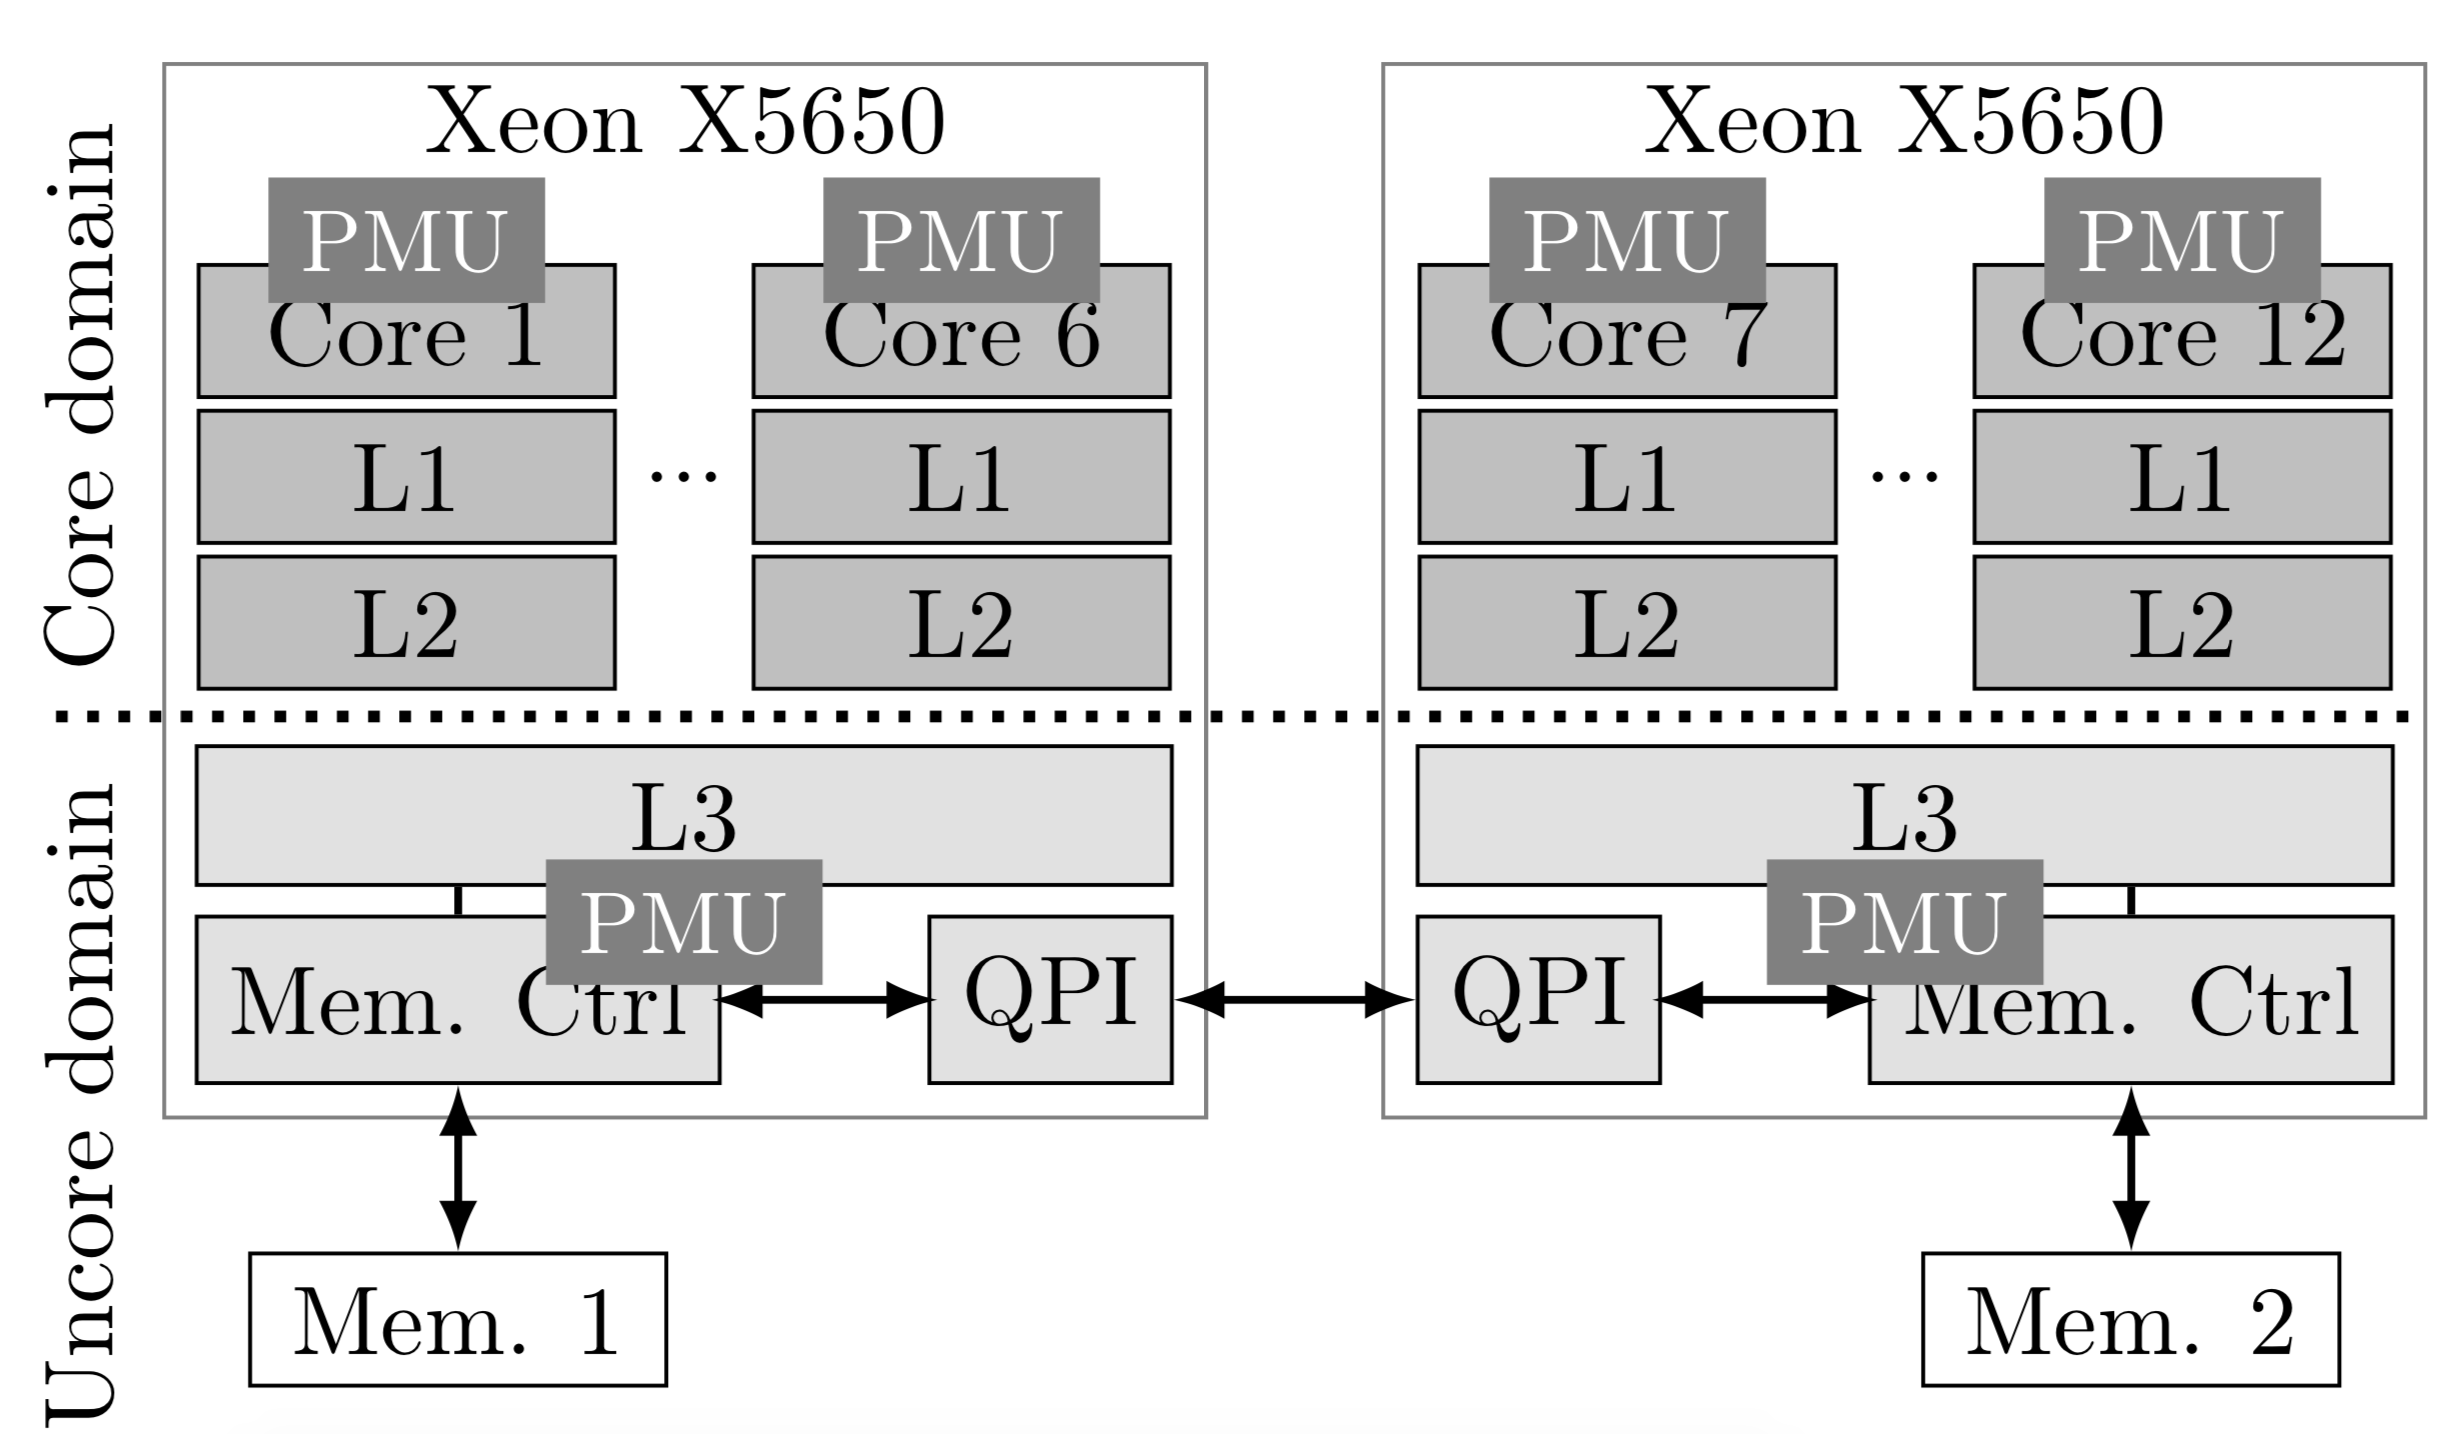
\includegraphics[width=10cm]{images/yamb_skl_pmu.png}
        \caption{\label{pic:yamb_skl_pmu}Exemple de disposition des PMU sur un processeur Skylake (extrait de \cite{Selva2017})}
        \end{figure}
        
        
        Pour pouvoir compter des évènements, la PMU doit être configurée à l'aide de registres matériels. Une PMU peut déclencher des interruptions qui nécessitent le support du noyau avant d'être converties en notification vers une application de niveau utilisateur, comme un signal par exemple. Pour ces raisons, l'accessibilité des compteurs est généralement très limité pour un utilisateur standard. Les PMU récente peuvent être configurées pour réaliser différente mesure. Les mesures peuvent être filtrées pour mesurer la totalité de l'activité ou seulement celle d'un processus. Ces configurations sont réalisés soit directement depuis le code (compilateur, manuellement) ou depuis le système (outils de profilage, noyeau). Les PMU peuvent être utiliser de deux façons différentes pour étudier l'activité d'un processeur: le comptage et l'échantillonnage. 
        
        \paragraph{Le comptage.} La première méthode consiste à compter le nombre d'évènements arrivant entre deux intervalles de temps. Pour cela, le compteur est initialisé à $0$ et lu au bout d'une certaine période de temps. Les valeurs ainsi récupérées permettent de mesurer le nombre d'occurrences de ces évènements. Cette méthode est efficace mais elle ne permet pas de connaître la partie du code responsable d'un évènement. Les ratio d'événements, tels que les instructions exécutées par cycle, les taux de \textit{miss} de mémoire cache et les taux d'erreurs de prévision des branches, peuvent être calculés en divisant le nombre par le temps écoulé.
        
        \paragraph{L'échantillonnage.} Pour obtenir plus d'informations sur le code responsable des évènements, le mode d'échantillonage ou \textit{sampling} doit être utilisé. Ce mode consiste déclencher une interruption tout les $n$ évènements et sauvegarder certaines informations tel que le pointeur d'instruction. Pour cela, le registre de comptage est initialisé à la valeur $MAX - n$ ou $MAX$ correspond à la valeur maximale pouvant être stocké dans le registre. Lorsque $n$ évènements sont compté, le registre déclenche un débordement (\textit{overflow}) et génère un exception traité par le système d'exploitation. Grâce à un échantillonage assez fin (nombre $n$ petit) et des méthodes de statistiques il est possible d'approcher le nombre d'évènements généré par chaque instruction. La principale difficulté de cette technique est d'assurer suffisamment de précision lors de l'attribution d'un évenement à une instruction. En effet, entre le moment ou l'interruption et généré et son traitement, plusieurs instructions peuvent avoir été exécutées. Des technologies telles que Intel PEBS\footnote{Documentation Intel - Intel 64 and IA-32 Architectures Software Developer’s Manual Volume 3B, Chapter 18. \url{https://software.intel.com/sites/default/files/managed/7c/f1/253669-sdm-vol-3b.pdf}} (Processor Event-Based Sampling) ou AMD IBS (Instruction Based Sampling) \cite{Drongowski2007} agrémentent le processeur d'un tampon lui permettant de stocker les informations nécessaires. L'autre avantage de cette technologie est de réduire l'impact sur les performances dû au traitement de chaque échantillon par le système d'exploitation. La PMU possède un tampon pouvant stocker plusieurs échantillons et n'interrompt l'exécution que lorsque ce tampon est plein. Le principale désavantage de cette technologie est le nombre restreint d'évènements compatible. De plus, elle n'est pas compatible avec toutes les architectures réduisant la portabilité des outils l'utilisant.
   
   \bigbreak

   Rappelle que le nombre de registre disponible est bien inferieur au nombre d’évèvenements disponible rendant impossible la collecte de tous les évenements à un moment donné. Pour cela, on a recourt a des techniques de multiplexages. De plus, certains évenement ne peuvent pas être mesuré en même temps pour des raisons architecturales.

   he idea behind multiplexing is to run several CPU hardware counter groups concurrently. This is accomplished by running the first CPU group for a short time interval, then switching to the next CPU group for the next short time interval. This is repeated in a round-robin fashion for the CPU groups until the event counting is eventually stopped.
   
   Multiplexing means that none of the specified CPU groups has been run on the whole code, and it is unknown what fraction of the code was measured with which group. It is assumed that the workload is sufficiently uniform that the measured event counts can be (more or less) safely calibrated as if the groups have been run separately on the whole code.
   
   Multiplexing consists
of scheduling events for a fraction of the execution and
extrapolating the full behavior of each metric from its
samples

Erreur de mutlipllexe \cite{Lim}
    
        
    \paragraph{TODO multiplexing} \textbf{1)}Simultaneously measuring more than four events requires multiplexing by regularly rotating the set of events that are active at each moment. This incurs some further overhead.
    \textbf{2)} When Hyper-Threading is disabled on modern Intel CPUs, however, the programmable counters of the unused hardware thread become available to the other – so there are eight available in total, per core



    \subsubsection{Compteurs matériels des architectures Intel}
    %%%%%%%%%%%%%%%%%%%%%%%%%%%%%%%%%%
        

        Pour mesurer les mesurer les évenements, les PMU des processeurs Intel possèdent deux types de compteurs: les \textit{Fixed-function counters} (FFC) et les compteurs de performance (HPMC). Les processeurs Intel possèdent une PMU \textit{uncore} directement sur le processeur et une PMU par coeur logiques, donc deux PMU par coeur physiques lorsque l'\textit{hyperthreading} est activé (voir \autoref{pic:edl_perf_pmu}). Chaque PMU \textit{oncore} possède 3 compteurs \textit{Fixed-Function} et 4 compteurs HPMC.
        
        \begin{figure}
        \center
        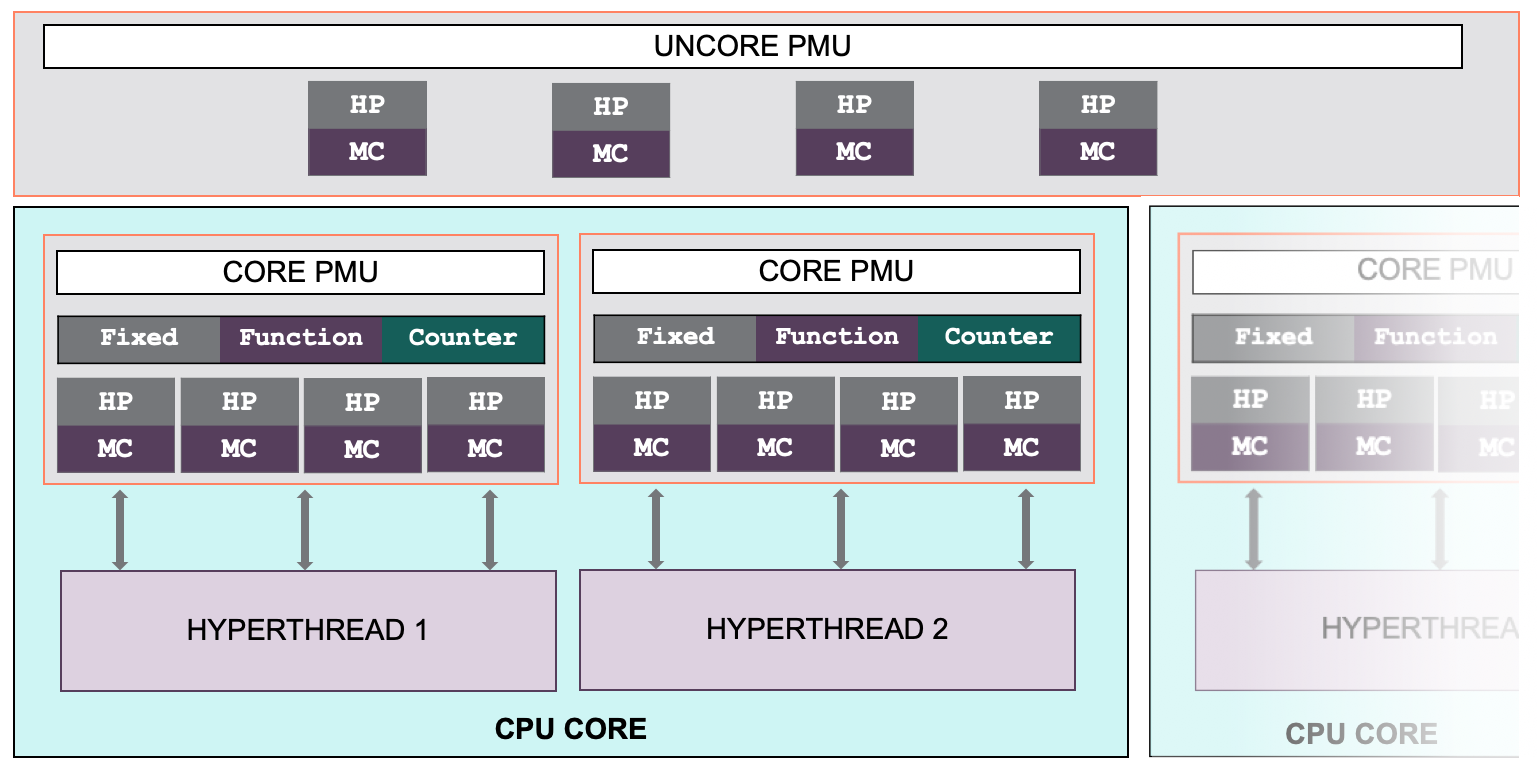
\includegraphics[width=12cm]{images/edl_perf_pmu.png}
        \caption{\label{pic:edl_perf_pmu} Dispositions des compteurs matériels sur un coeur d'un processeur Intel.}
        \end{figure}
    
        %%%%%%%%%%%%%%%%%%%%%%%%%%%%%%%%%%%%%%%%%%%%%%%%%%%%%%%%%%
        \paragraph{Les compteurs FFC}
        Les compteurs \textit{Fixed-Function} sont les plus simples à utiliser car ils sont déjà configurés pour compter un évènement. Sur les architectures Intel, il y a 3 compteurs FFC par coeur logique. Le premier compteur (\textit{IA32\_FIXED\_CTR0}) compte le nombre d'instruction exécutée par un coeur. Le deuxième (\textit{IA32\_FIXED\_CTR1}), compte le nombre de cycle à la fréquence nominale du processeur. Enfin le troisième (\textit{IA32\_FIXED\_CTR3}), compte le nombre de cycle durant lequel le coeur est actif. Pour pouvoir utiliser ces trois compteurs, une simple configuration est requise grâce aux deux registres \textit{IA\_32\_PERF\_GLOBAL\_CTRL} et \textit{IA\_ Le 32\_FIXED\_CTR\_CTRL} (voir \autoref{pic:edl_perf_ffc}). 
        
        \begin{figure}
        \center
        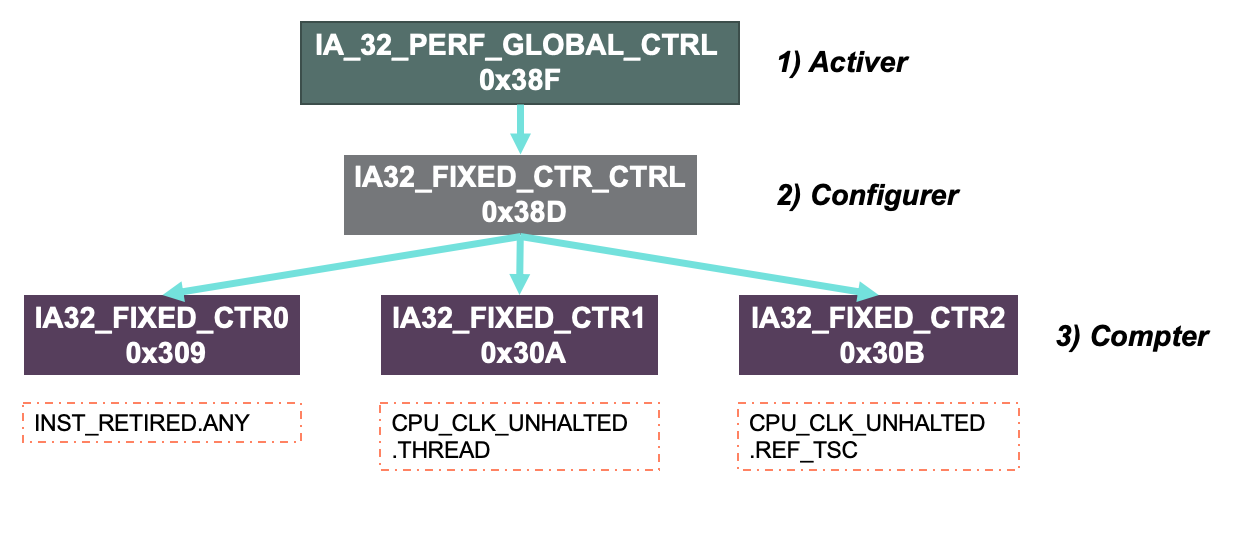
\includegraphics[width=10cm]{images/edl_perf_ffc.png}
        \caption{\label{pic:edl_perf_ffc} Chaque coeur logique dispose d'une PMU possédant 3 compteurs pré-configuré pour compter un type d'évènement.}
        \end{figure}
        
        
        Le premier MSR permet d'activer les deux types de compteurs (HPMC et PPF). Chaque bit de ce registre correspond à l'activation ou non du compteur associé. Cette activation n'a à être réalisé qu'une seul fois au démarrage du processeur. Le deuxième registres permet quand à lui de configurer le comptage d'évenement: mode utilisateur ou noyau, mesure du coeur logique associé ou de tout le coeur physique, et si le compteur doit générer ou non un interruption lorsque celui-ci dépasse la valeur maximale pouvant être stocké sur 48 bits. Ce dernier bit de configuration peut être utilisé pour vérifier l'utilisation ou non du compteur par un autre programme (qui voudrait être alerté par une interruption. Une fois ces deux opérations réalisés (activation et configuration), les évènements sont compté dans les trois registres correspondant, il ne suffit alors plus que de lire la valeur s'y trouvant. Bien qu'il ne soit pas nombreux, les trois compteurs FFC permettent d'obtenir des informations interessante sur l'utilisation du processeur. Par exemple en divisant le troisième compteur par le deuxième ($\frac{IA32\_FIXED\_CTR3}{IA32\_FIXED\_CTR2}$) on obtient le pourcentage d'utilisation du coeur. En utilisant le premier compteur on peut aussi obtenir un bon indicateur sur la performance du code: le nombre d'instruction exécutées chaque cycle.
        
       
        
        
        %%%%%%%%%%%%%%%%%%%%%%%%%%%%%%%%%%%%%%%%%%%%%%%%%%%%%%%%%%%%%%%%%%%
        \paragraph{Les compteurs HPMC.} Les compteurs HPMC sont plus difficile à utiliser car il doivent être configurer par l'utilisateur et la longue documentation (plusieurs centaines de pages) n'est pas toujours évidente à comprendre. Les compteurs HPMC sont présent sur les PMU des \textit{oncore} et \textit{uncore}. Leur nombre dépend de l'architecture, les derniers processeurs Skylake possèdent 4 compteurs HPMC par PMU \textit{oncore}, donc 8 compteurs par coeur. Un compteur HPMC est composé de deux registres. L'un est utilisé pour la configuration, le deuxième pour le comptage (voir \autoref{pic:edl_perf_hpmc}).
        
       \begin{figure}[h!]
        \center
        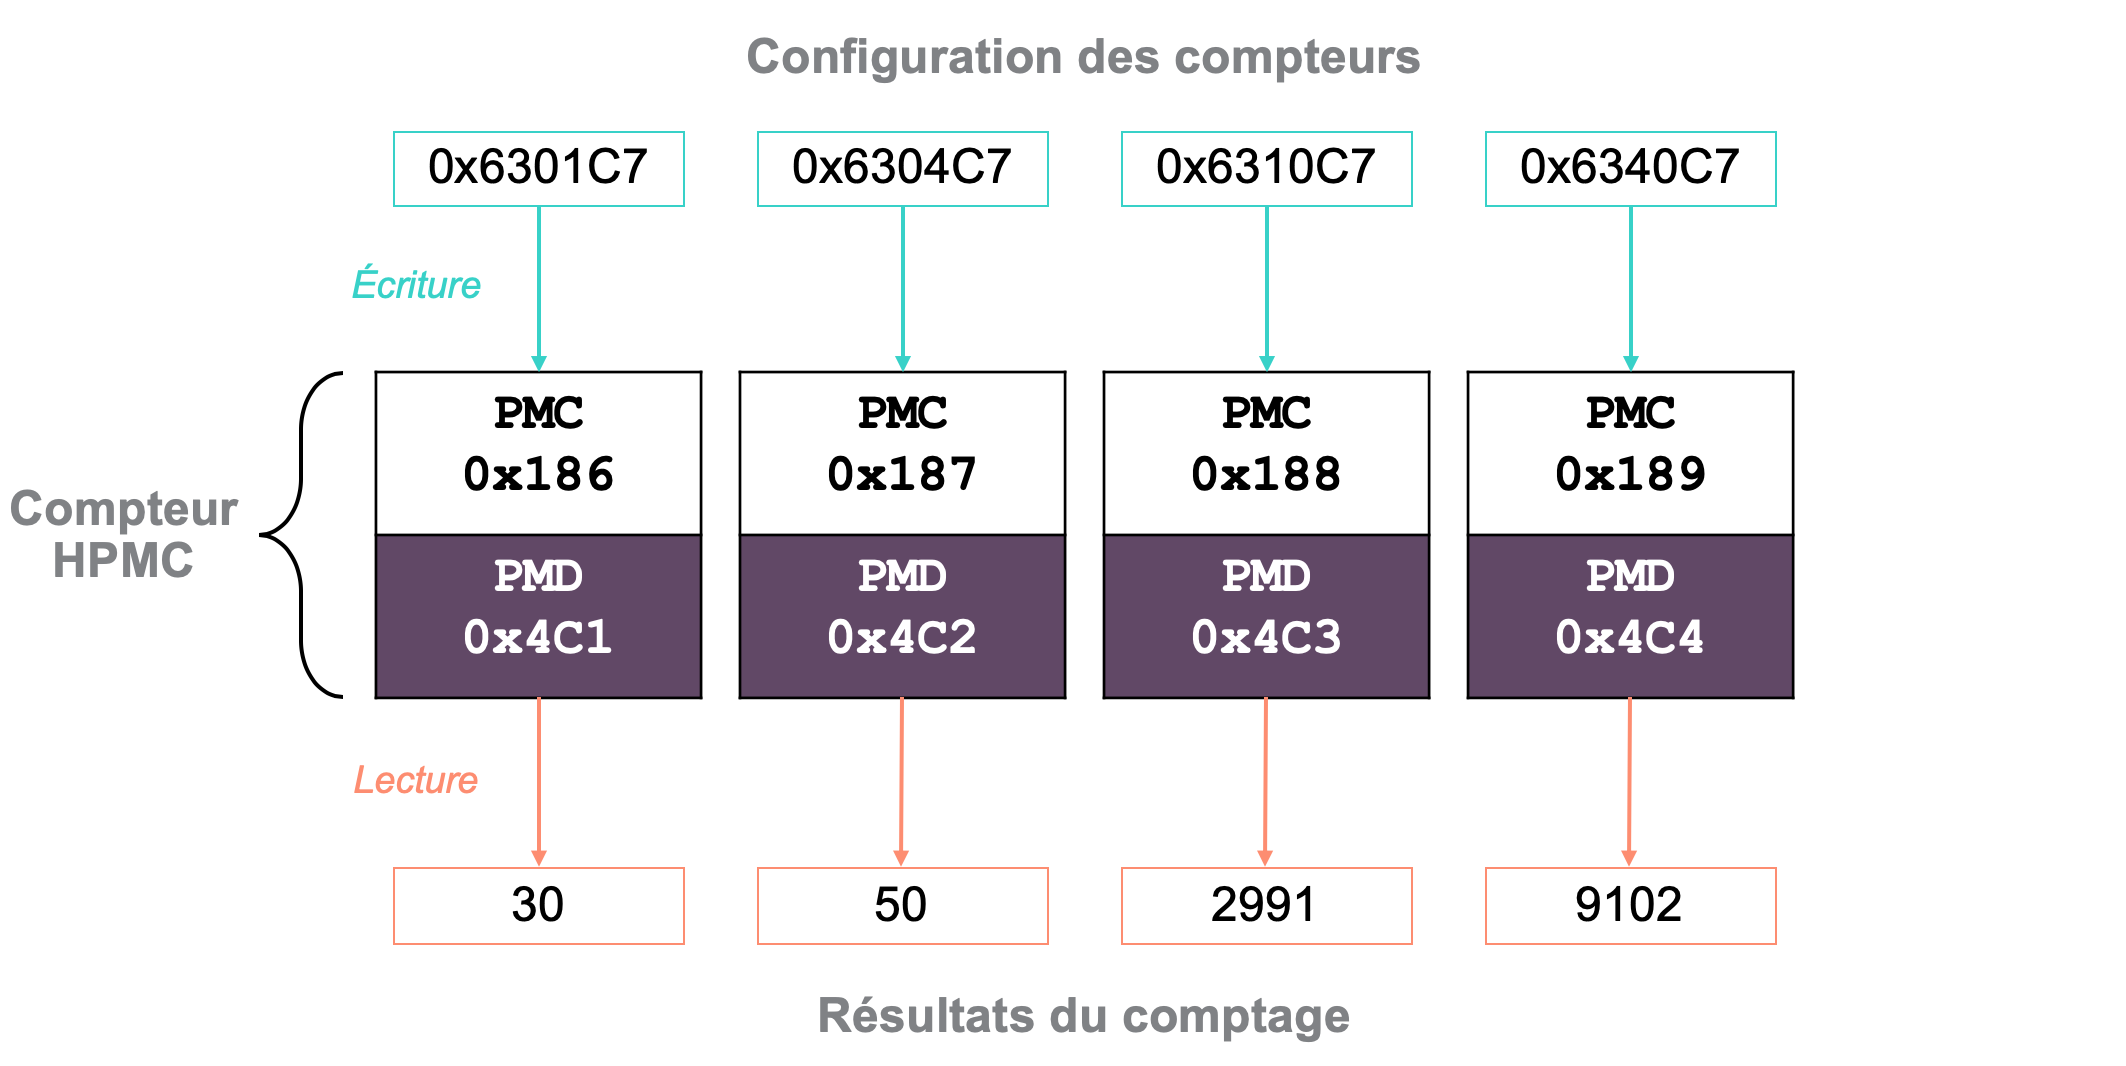
\includegraphics[width=14cm]{images/edl_perf_hpmc.png}
        \caption{\label{pic:edl_perf_hpmc} Chaque coeur logique dispose d'une PMU possédant 4 compteurs HPMC pouvant être configurés pour compter différent évènements. Dans cet exemple, les 4 compteurs sont configurés pour compter toutes les opérations flottante en double précisions exécutés sur le coeur (opérations scalaires et vectorielles (128, 256 et 512 bits)).}
        \end{figure}
        
        Le premier registre est appelé PMC (Performance Monitoring Controler) référencé sous le nom \verb|IA32_PERFEVTSELx|. Chaque HPMC possède son propre registre PMC (accessibles aux adresses 0x186, 0x187, 0x188 et 0x189) qui permet de réaliser la configuration du compteurs: activation, génération d'un interruption, mode (utilisateur ou noyau), évènement à compter (voir \autoref{pic:eld_perf_pmc}). Le \autoref{tab:pmc_config} montre un exemple de configuration d'un compteur pour compter le nombre instructions flottante scalaire exécutée. Il faut pour cela trouver le code correspondant dans la documentation Intel \cite{Intel2018} au chapitre 19.2 pour les évènements Skylake. Ensuite les différents bits de configuration sont utilisés pour activer le compteur, compter les évènements pour le système d'exploitation et l'utilisateur de tout les threads exécutés sur ce coeur. La valeur résultante (\verb|0x6301C7|) n'a plus qu'à être écrite dans un des quatre MSR du coeur pour lancer le comptage dans le registre PMD correspondant.
        
        Le deuxième registre des compteurs HPMC est appelé PMD (Performance Monitoring Data). Il enregistre le nombre d'évènement depuis sont activation réalisée avec registre PMC qui lui est associé. Ces MSR sont des registres architecturaux nommés \verb|IA32_PMC| localisé des adresses \verb|0x4C1| à \verb|0x4C4|.
       
        
        % Please add the following required packages to your document preamble:
        % \usepackage{graphicx}
        \begin{table}[]
        \centering
        \begin{tabular}{l|c|c|c|c|c|c|c|c|c|c|c|}
        \cline{2-12}
        & \multicolumn{1}{l|}{CMASK} & \multicolumn{1}{l|}{INV} & \multicolumn{1}{l|}{EN} & \multicolumn{1}{l|}{ANY} & \multicolumn{1}{l|}{INT} & \multicolumn{1}{l|}{PC} & \multicolumn{1}{l|}{E} & \multicolumn{1}{l|}{OS} & \multicolumn{1}{l|}{USR} & \multicolumn{1}{l|}{UMASK} & \multicolumn{1}{l|}{EVENT} \\ \hline
        \multicolumn{1}{|l|}{bits} & 31 - 24 & 23 & 22 & 21 & 20 & 19 & 18 & 17 & 16 & 15 - 08 & 7 - 0 \\ \hline
        \multicolumn{1}{|l|}{Valeur} & 0 & 0 & 1 & 1 & 0 & 0 & 0 & 1 & 1 & 1 & C7 \\ \hline
        \multicolumn{1}{|l|}{Résultat} & 0 & \multicolumn{4}{c|}{6} & \multicolumn{4}{c|}{3} & 1 & C7 \\ \hline
        \end{tabular}%
        \caption{Configurer un compteur pour compter le nombre d'instruction flottantes exécutées revient à écrire la valeur $0x6301C7$ dans son registres PMC.}
        \label{tab:pmc_config}
        \end{table}
        
        \begin{figure}
        \center
        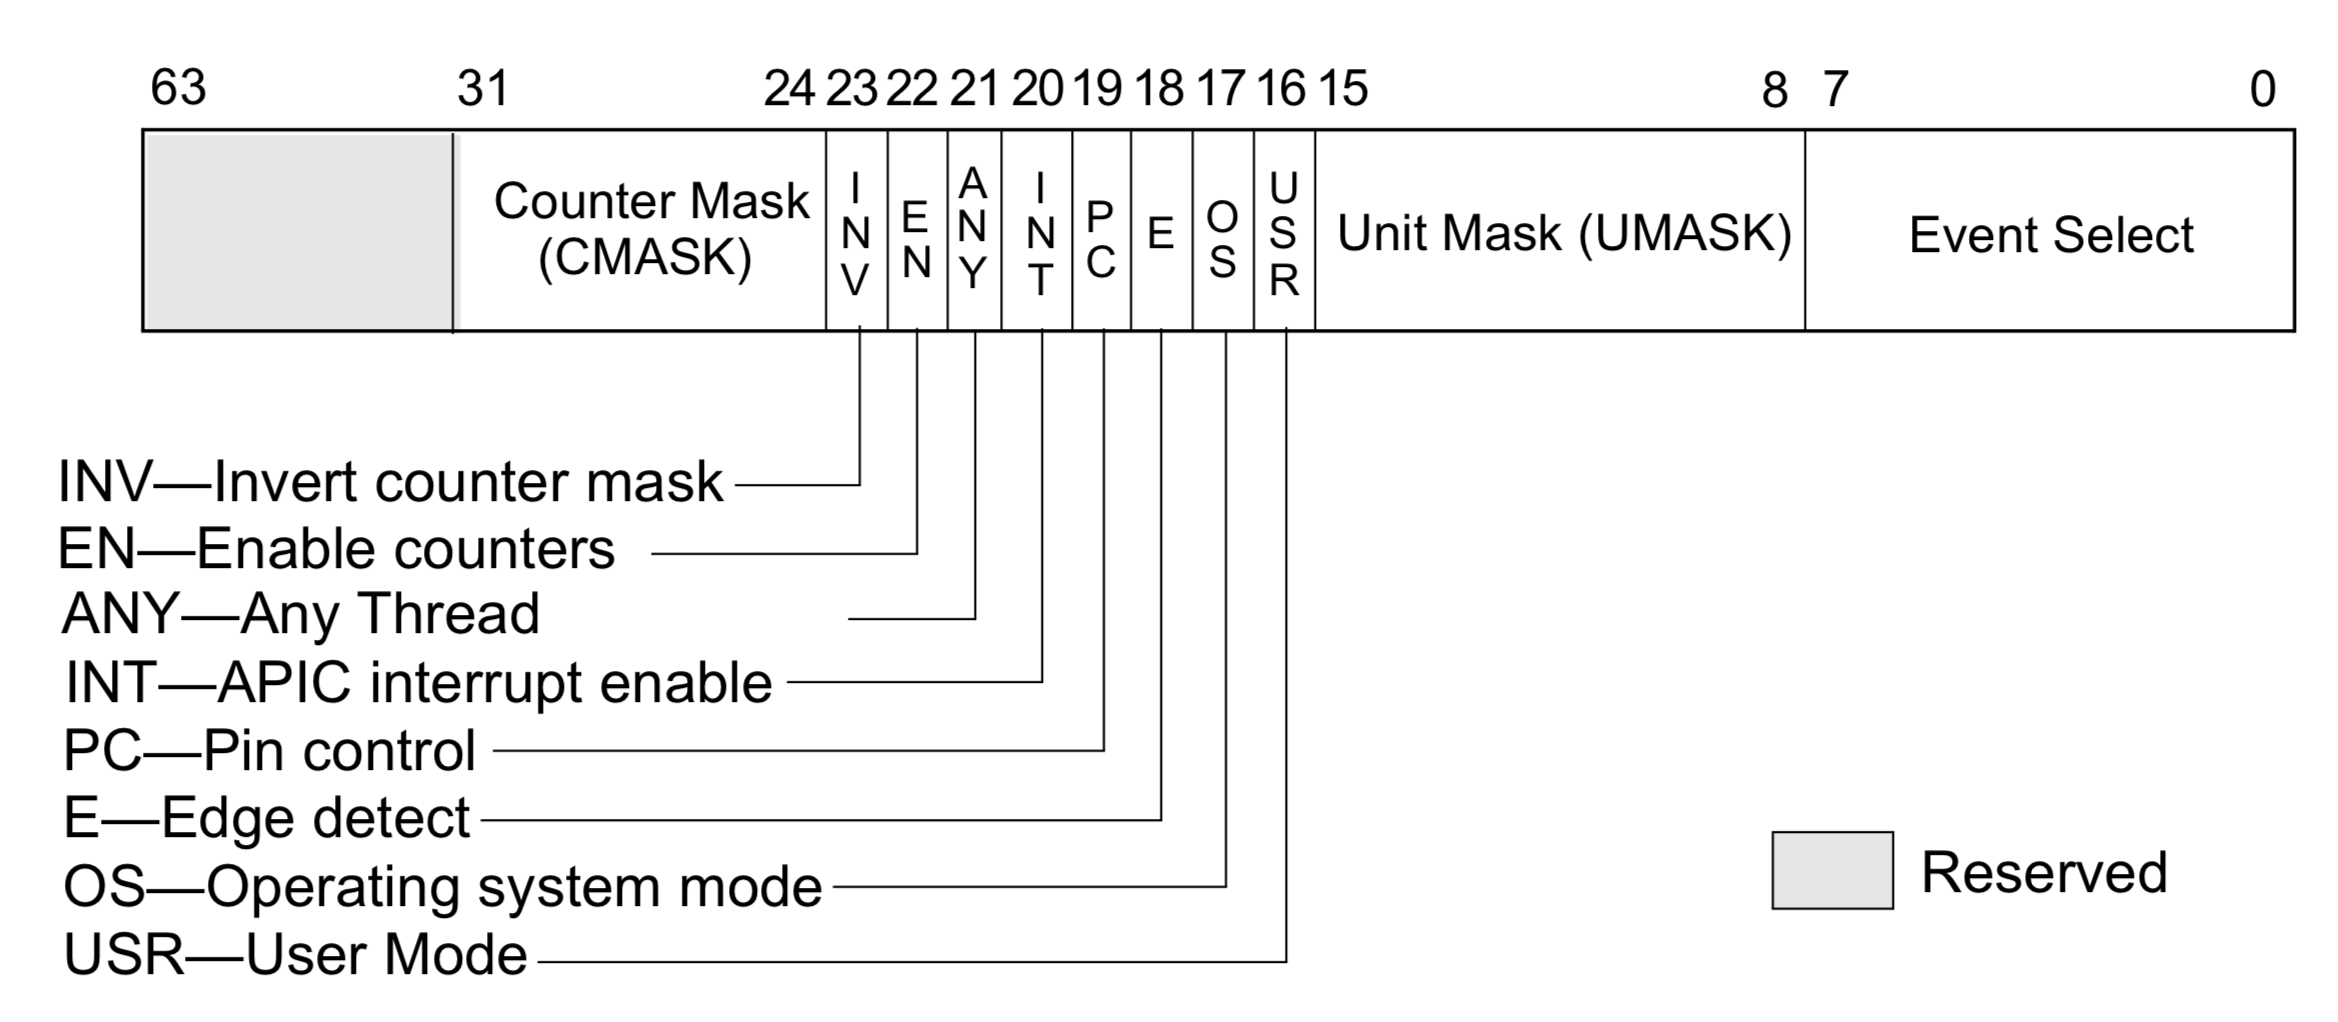
\includegraphics[width=10cm]{images/eld_perf_pmc.png}
        \caption{\label{pic:eld_perf_pmc}}
        \end{figure}

        
        
               
    \subsubsection{Programmation des compteurs en assembleur} \label{sec:perf_asm_msr}
    %%%%%%%%%%%%%%%%%%%%%%%%%%%%%%%%%%
    
        Au fil des générations, les architectures ont reçus plusieurs instructions permettant d'interagir avec les registres MSR. Les processeurs Intel possèdent actuellement 5 instructions nécessitant différents privilèges pour les exécuter (voir \autoref{fig:edl_perf_assembly_msr}).
        
        \begin{figure}[h!]
            \center
            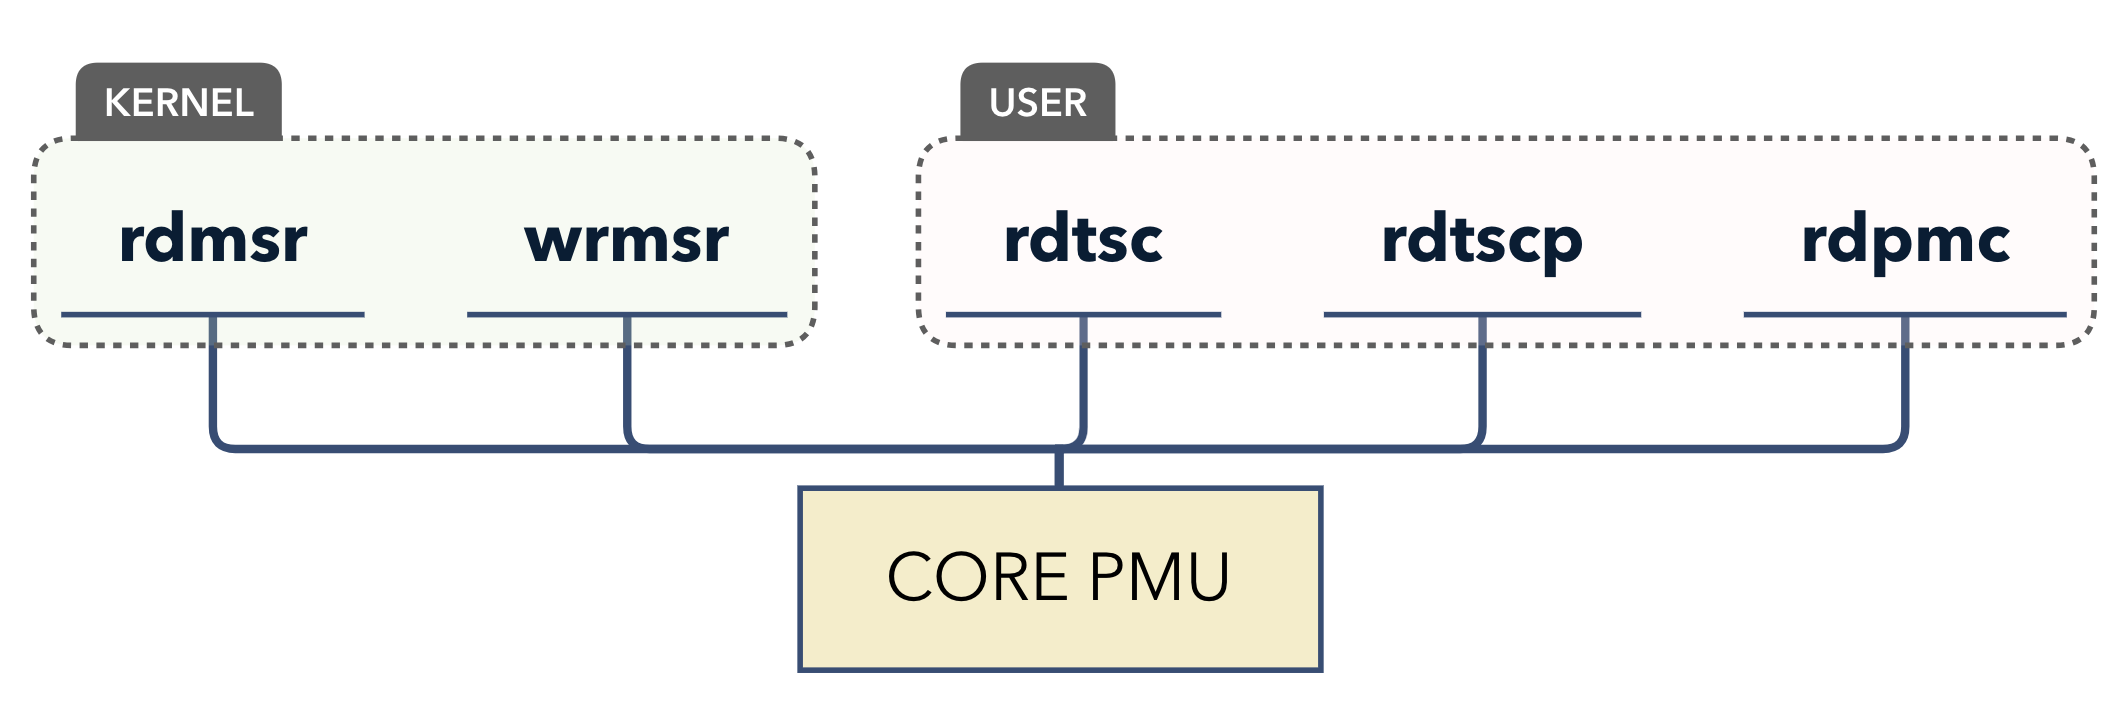
\includegraphics[width=10cm]{images/edl_perf_assembly_msr.png}
            \caption{\label{fig:edl_perf_assembly_msr} Instructions assembleurs permettant d'accéder aux registres MSR d'une architecture Intel.}
        \end{figure}
    
    
        Les compteurs sont des registres matériels, ils peuvent donc être écrit et lu comme n'importe quel autre registre. Il existe deux instructions assembleur permettant d'écrire (\textit{wrmsr}) et de lire (\textit{rdmsr}) ces registres. Les registres accessibles à l'utilisateur peuvent être listés grâce à l'instruction \textit{cpuid}. Cependant, ces instructions ne peuvent être exécutés que par un processus de privilège 0. En effet, laisser la possibilité à un utilisateur normal de modifier ces registres peut être très dangereux pour la sécurité du système. Tout les processus qui veulent intéragir avec les registres MSR doivent donc pouvoir accéder à ce niveau de privilège. C'est \textit{la} contrainte majeur qui rend difficile le développement d'outils de suivi de performance. De multiples moyen ont été mis au point depuis pour pouvoir y accéder sans compromettre la sécurité du système. 
        
        Le premier moyen a été introduit par Intel grâce à la création d'une troisième instruction assembleur permettant de lire le contenu d'un registre avec l'instruction \textit{rdpmc}. Cette instruction a ajouté avec la sortie du Pentium Pro en 1995. Bien que cette instruction ne permette par d'écrire dans un registre, elle permet de lire le résultat des compteurs et notamment les compteurs FFC. Ces compteurs étant déjà configurés, l'instruction \textit{rdpmc} permet de pouvoir lire ces trois compteurs sans privilège supplémentaire. Dans un programme C, le compteur \textit{ctr} (1, 2 ou 3) peut être lû grâce au code de l'\autoref{lst:edl_rdpmc_ffc}. L'instruction \textit{rdpmc} peut aussi être utilisé pour lire les compteurs HPMC grâce au code de l'\autoref{lst:edl_rdpmc_pmc}. Cela peut être utile pour laisser les utilisateurs accéder aux résultat des compteur HPMC après qu'un autre programme ayant les droits d'utilisation de l'instruction \textit{wrmsr} ait paramétré les compteurs.
    
    
    

\begin{minipage}{.50\textwidth}
\begin{lstlisting}[
label=lst:edl_rdpmc_ffc,
basicstyle={\scriptsize\ttfamily},
identifierstyle={\color{black}},
language={c},
tabsize=2,
numbersep=8pt,
frame=tlbr,framesep=2pt,framerule=0pt,
morekeywords ={class,run},
caption=Boucle déroulée 4 fois.
]
ul rdpmc_Fixed-Function (int ctr){
   unsigned a, d, c;
   c = (1<<30) + ctr;
   __asm__ volatile("rdpmc" : "=a" (a), 
                              "=d" (d) 
                            :  "c" (c));
   return ((unsigned long)a) | 
         (((unsigned long)d) << 32);;
}
\end{lstlisting}
\end{minipage}%%
\hfill
%&
%
\begin{minipage}{.50\textwidth}
\begin{lstlisting}[
label=lst:edl_rdpmc_pmc,
basicstyle={\scriptsize\ttfamily},
identifierstyle={\color{black}},
tabsize=2,
language={c},
numbersep=8pt,
xleftmargin=0.5cm,frame=tlbr,framesep=2pt,framerule=0pt,
morekeywords ={class,run},
caption=Boucle déroulée 16 fois.
]
ul rdpmc_counter (int ctr){
   unsigned a, d, c;
   c = ctr;
   __asm__ volatile("rdpmc" : "=a" (a), 
                              "=d" (d) 
                            :  "c" (c));
   return ((unsigned long)a) | 
         (((unsigned long)d) << 32);;
}
\end{lstlisting}
\end{minipage}


\subsection{Interfaces pour accéder aux PMU}
%%%%%%%%%%%%%%%%%%%%%%%%%%%%%%%%%%
    
    
    La section précédente présente les PMU des processeurs Intel, les différents compteurs disponibles ainsi que la façon d'y accéder en assembleur. Interagir avec des registres matériels n'est possible qu'en utilisant les instructions assembleurs présentés ci-dessus. Cependant, cette méthode est très difficile pour le développement d'outils sophistiqués. Ainsi, différentes interfaces à ces instructions ont été développés. La quasi-totalité des supercalculateurs HPC (100\% du Top500) utilisent un système d'exploitation basé sur le noyau linux. Nous nous intéressons dans cette partie au différents moyens disponibles lors de l'écriture de cette thèse pour utiliser les compteurs qui sont compatibles avec cet environnement. Le support par Linux des compteurs matériels a été long empêchant les développeurs de construire des outils facilement portables. Pour ce faire, différents patch logiciels devait être appliqués noyau pour supporter leur utilisation: perfctr \cite{Pettersson2005} ou les projets perfmon et perfmon2 \cite{Eranian2006}, développés par Stéphane Eranian, ancien employé HP. En 2009, la prise en charge des compteurs de performance a finalement été fusionnée dans le noyau Linux, en tant que projet Performance Counters for Linux (PCL) rebaptisé \textit{Perf Events}.

    
    Cette section présente les différentes façons d'utiliser les compteurs des architectures Intel, présentés dans la section précédente. La présentation commence par la outils de plus bas niveau pour ensuite présenter les outils plus haut niveau.
 
 
    \subsubsection{Pseudo système de fichier /dev/cpu/CPUID/msr}
    %%%%%%%%%%%%%%%%%%%%%%%%%%%%%%%%%%
    La première solution est implémenté par le noyau Linux permettant à l'utilisateur un accès bas niveau aux MSR sans avoir à utiliser de langages assembleurs. Ceci est réalisé à travers un pseudo système de fichier permettant d'intéragir avec tous les coeurs (identifié par leur \verb|CPUID|) à travers le chemin \verb|/dev/cpu/#CPUID/msr|. Par défaut, seul l'utilisateur \textit{root} est autorisé à modifier ce fichier, mais ses droits peuvent être modifié pour étendre l'accès aux autres utilisateurs. L'utilisation de cette interface est très pratique et peut être réalisée en accédant au fichier \textit{msr} grâce aux opérations \verb|pread()| et \verb|pwrite()|. Par exemple, pour lire le MSR dont l'adresse est \verb|0x38|, il suffit d'ouvrir le fichier \textit{msr} correspondant au coeur voulu, et réaliser une lecture avec un décalage de 38 octets.
    
    \begin{figure}[h!]
    \center
    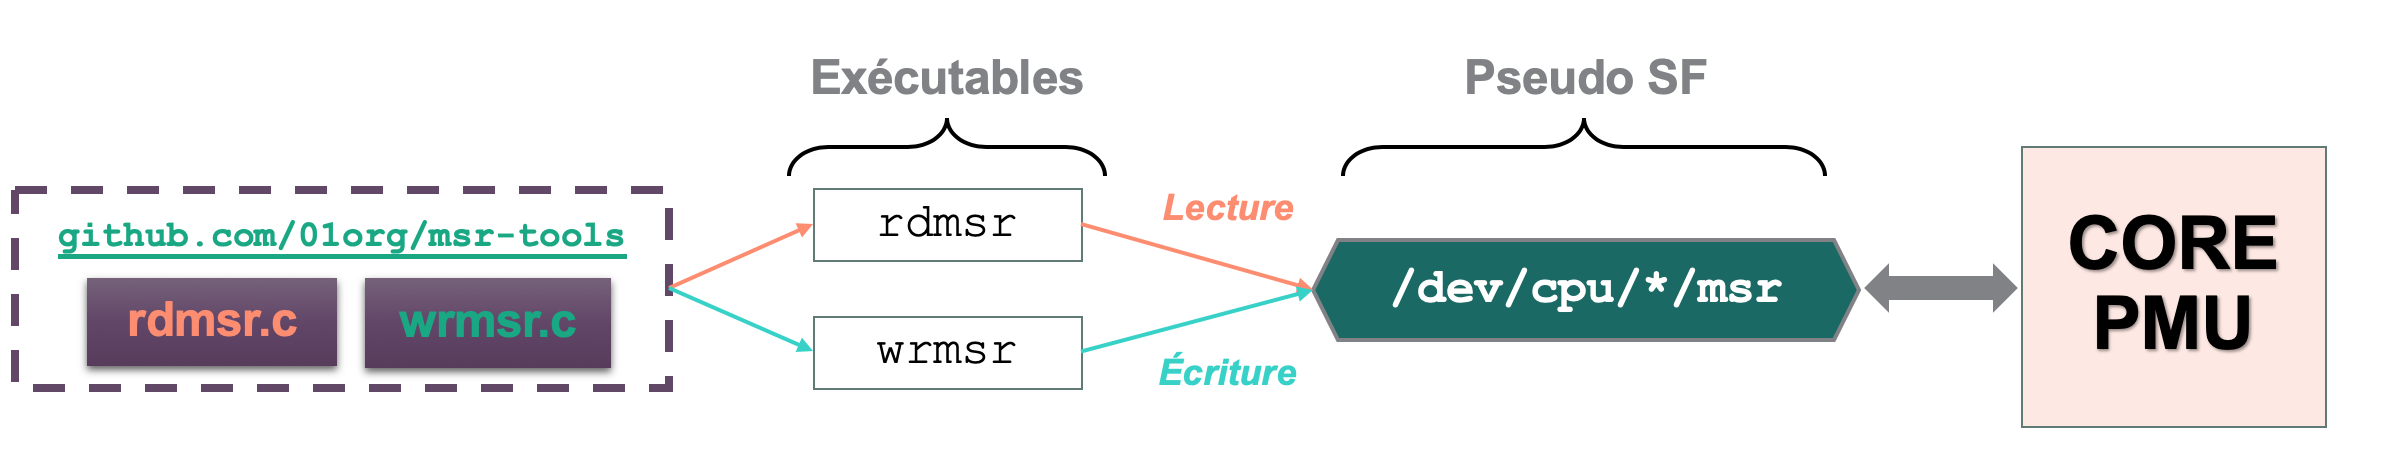
\includegraphics[width=14cm]{images/edl_perf_msrtools.png}
    \caption{\label{fig:edl_perf_msrtools} Intel propose deux exécutables permettant d'interagir plus facilement avec le pseudo système de fichier.}
    \end{figure}

    Pour faciliter l'usage de l'interface, Intel propose l'outil \textit{msr-tools} sur son GitHub\footnote{\url{https://github.com/intel/msr-tools}} (voir \autoref{fig:edl_perf_msrtools}).  La compilation produit deux exécutables \verb|rdmsr| et \verb|wrmsr| qui permettent de réaliser les lectures et écriture des registres MSR comme cela: \verb|./rdmsr -r 0x38D|. Nous proposons dans notre travail trois scripts permettant d'initialiser et configurer les compteurs grâce à ces deux programmes\footnote{\url{https://github.com/PourroyJean/performance_modelisation/tree/master/src/tool_PMU}}. 
    
    
    \subsubsection{Perfmon2}
        Le projet perfmon2 était le principal candidat à l'inclusion dans le noyau Linux avant l'émergence surprise de \textit{Perf Events}. L'objectif du projet perfmon2 est de concevoir une interface générique de suivi des performances de bas niveau pour accéder à toutes les implémentations d'unités de surveillance des performances matérielles (PMU).
        
        L'interface est constituée de l'appel système perfmonctl. Un appel système a été préféré à un driver de périphérique car il offre une plus grande flexibilité et facilite la prise en charge par les implémentations d'un mode de surveillance par thread qui nécessite d'enregistrer et de restaurer l'état PMU du thread. L'interface exporte tous les registres PMU comme des registres 64 bits, même si de nombreuses implémentations PMU Interfaces en ont moins. L'interface ne sait pas ce que fait chaque registre, combien il y en a, ni comment ils sont associés les uns aux autres. L'implémentation pour chaque plate-forme met en correspondance les PMC et PMD logiques sur les registres PMU réels. Toutes les informations spécifiques à un événement sont reléguées au niveau de l'utilisateur où elles peuvent être facilement encapsulées dans une bibliothèque.
    
        Le code de perfmon2 n'a jamais réussi a être inclus dans le projet Linux et son développement a été arrété suite à la présentation du projet concurrent \textit{Perf Events}.
    
    
    
    \subsubsection{Perf Events}
    %%%%%%%%%%%%%%%%%%%%%%%%%%%%%%%%%%
        
        Le projet de Compteur de Performance pour Linux (PCL) a été présenté en décembre 2008 et introduite dans Linux 2.6.31. Cet outil, rebaptisé ensuite \textit{Perf Events}, est une réponse au projet principale de standardisation des compteurs pour Linux de l'époque: perfmon2. Alors que ce dernier présentait beaucoup de fonctionnalités intéressantes, il n'a jamais réussi à être inclu dans le projet Linux pour des raisons pas forcément techniques... Lorsque \textit{Perf Events} fût ajouté au noyau Linux, de nombreuses fonctionnalité manquait mais sont apparût depuis. Pour fonctionner, \textit{Perf Events} utilise son interface \textit{perf\_event} développé directement dans le code du noyau Linux. Son adoption dans le noyau a mis un frein aux développement d'autres interfaces telle que \textit{perfmon2} ou \textit{perfctr} qui nécessitait de patcher le noyau pour pour être utilisée.  Du projet \textit{perfmon2}, seul la librairie \textit{libpfm4} est encore active. Il s'agit d'une librairie qui permet de convertir les nom symboliques d'évènements PMU en leur encodage pour \textit{Perf Events} ou d'autre interface noyau (exemple de la \autoref{fig:edl_perf_libpfm4}). La librairie en elle-même ne mesure aucun évènement. Elle fournit aux développeurs une interface pour lister, encoder les évènements pour beaucoup de PMU (core et uncore).
        
        \begin{figure}[h!]
        \center
        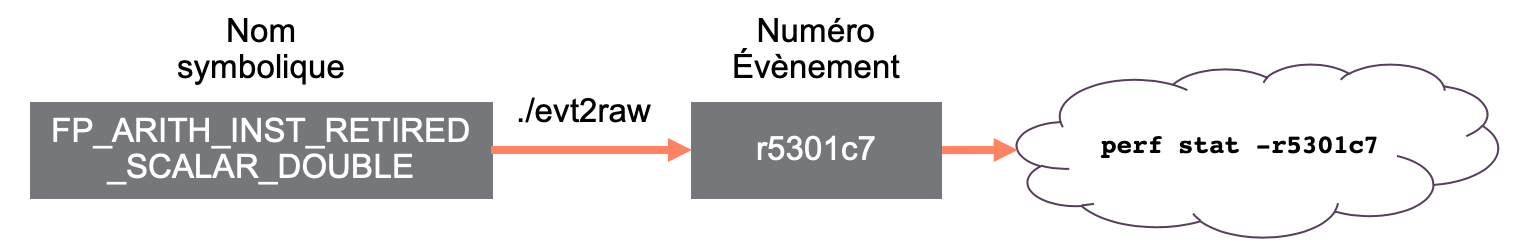
\includegraphics[width=12cm]{images/edl_perf_libpfm4.png}
        \caption{\label{fig:edl_perf_libpfm4} \textit{Libpfm4} permet de convertir les noms symbolique des évènements en leur encodage correspondant pouvant être utilisé avec des outils tels que \textit{perf}.}
        \end{figure}
        
        
        Un point de désaccord persistant entre \textit{Perf Events} et d'autres approches (tel que \textit{perfmon2}) est qu'il incorpore toutes les informations sur les compteurs et les événements dans le code du noyau lui-même, ajoutant ainsi une quantité significative de code descriptif au noyau. L'intégration de telles données dans le noyau peut causer des difficultés aux outils utilisateur pour prendre des décisions sur les événements qui peuvent être comptés simultanément et aux fournisseurs pour fournir des mises à jour sans avoir à patcher le noyau ou attendre de nouvelles versions du noyau.
        
        
        introduit un seul appel système comme point d'entrée à une seule abstraction de compteur. L'appel, \textit{sys\_perf\_open}, renvoie un descripteur de fichier qui donne accès aux événements matériel. 
        
    
        \paragraph{perf.} 
        En plus de l'appel système, \textit{Perf Events} fournit un outil accessible depuis l'espace utilisateurs lui permettant de contrôler le profilage. Nommé \textit{perf}, ce programme utilise l'interface noyau pour réaliser des mesures soit en échantillonage soit en comptage. Différentes commandes sont disponibles pour compter les évènements (\textit{stat}, \textit{record}, \textit{top}, \textit{bench}) et afficher les résultats (\textit{report}, \textit{annotate}). Grâce à la commande \textit{perf}, il est possible de compter les évènements en utilisant directement leur nom. La commande suivante peut être utilisée pour mesurer le nombre de transaction en lecture réalisée par un contrôleur mémoire. Il faut pour cela, vérifié que le noyau utilisé est capable d'accéder aux PMU uncore (première commande ci dessous). Ensuite, il faut vérifier que le noyau supporte l'utilisation des noms d'évènements symbolique (deuxième commande ou \verb|perf list|). Enfin, la troisième commande permet de compter le nombre d'évènement.
        
\begin{verbatim}
#ls /sys/bus/event_source/devices/* | grep uncore_imc
uncore_imc_0 uncore_imc_1 uncore_imc_3 uncore_imc_4 uncore_imc_5

#ls /sys/bus/event_source/devices/uncore_imc_1/events/
cas_count_read  cas_count_read.scale  cas_count_read.unit clockticks ...         

#perf stat –a -e uncore_imc_0/cas_count_read/
\end{verbatim}
        
        Malheureusement, lorsque les évènements voulus ne sont pas supportés par le noyau, il est nécessaire de se reporter à la documentation de l'architecture. Perf (comme PAPI) est capable de configurer les compteurs grâce à leur encodage (numéro de l'évènement, masque de configuration). Dans notre exemple, l'évènement est le numéro $0x04$ associé au masque $0x03$. Lorsque l'évènement est supporté par le noyau, c'est cette valeur qui est stockée dans les fichiers listés ci-dessus (première commande). Pour réaliser le même comptage que précédemment, la deuxième commande ci dessous peut être utilisée:
        
\begin{verbatim}
# cat /sys/bus/event_source/devices/uncore_imc_1/events/cas_count_read
event=0x04,umask=0x03

#perf stat -a -e "uncore_imc_0/event=0x04,umask=0x03/"
Performance counter stats for 'system wide':
	4.94 MiB  uncore_imc_0/cas_count_read/
\end{verbatim}


        \paragraph{Avantages.} Bien qu'il s'agisse avant tout d'un outil d'espace utilisateur, la commande perf fait partie du noyau Linux du point de vue du développement. Faire partie de Linux assure une haute exigence du développement du code ainsi qu'un support au fil des versions du noyau. Lorsque le noyau supporte le nom symbolique des évènements, \textit{perf} est très simple à utiliser. Dans le cas contraire, \textit{Perf Events} offre la possibilité aux utilisateurs expérimentés d'encoder leurs propres évènements.
        

        \paragraph{Inconvénients.} L'inclusion de \textit{Perf Events} au projet Linux peut aussi être un inconvénient en rendant l'outil intrinsèquement lié à la version du noyau Linux. Ceci implique que pour utiliser les nouvelles fonctionnalités de perf il faut généralement installer la version du noyau correspondante. La deuxième difficulté vient de l'appel système \textit{perf\_event\_open}. S'il permet d'éviter à l'utilisateur d'écrire manuellement les différents bits de configuration des MSR, beaucoup de travail reste à faire pour le développeur désireux de profiler ses applications. Parce que Linux supporte de nombreux processeurs différents possédant différentes version de PMU, les développeurs de noyau ont dû laisser la charge de beaucoup de détails de micro-architecture de bas niveau dépendant du code utilisateur. En conséquence, cet appel système est très complexe à utiliser et ne peut pas être utilisé de manière portable. Les principales difficultés consistent à trouver les événements à compter ou à échantillonner, à configurer tous les paramètres à transmettre à l'appel système et à effectuer plusieurs appels système en fonction du nombre de \textit{threads} de l'application profilée et du nombre de coeurs utilisés. Ces différentes difficultés (programmation, portabilité) ont été les principales motivations du développement d'autres outils tels que PAPI, Intel Performance Counter Monitor (PCM) ou NUMAP\cite{Selva2017}.


    \subsubsection{Oprofile.} 
    %%%%%%%%%%%%%%%%%%%%%%%%%%%%%%%%%%
        Oprofile \cite{Levon2004} est un outil de suivi de performance développé par John Levon en 2001 dans le cadre de son projet de master et fut le principale outil de suivi de performance de Linux pendant plusieurs années\footnote{source: \url{https://www.ibm.com/developerworks/linux/library/l-evaluatelinuxonpower/}}. 
        Oprofile est capable d'utiliser des compteurs de performances matérielles pour suivre la performance des processus, des bibliothèques partagées et du noyau. Pour suivre ces performances, Oprofile utilise un démon permettant à l'utilisateur de spécifier un événement matériel à surveiller et un seuil d'événement pour déclencher l'interruption (échantillonage). En utilisant les tables de symboles de débogage, il peut faire le lien entre les adresses des instructions et les lignes du code source associées. Oprofile est un outil mature possédant une multitude d'option telle que la génération de graphiques d'appel (\textit{call graph}). Plusieurs utilitaires sont fournis à l'utilisateur pour contrôler le suivi de performance (\textit{opcontrol}, \textit{opreport} ...).
        A l'origine, Oprofile utilisait un module noyau nécéssaire pour accéder aux PMU. Quand \textit{Perf Events} fut introduit avec son interface noyau, Oprofile a alors été adapté pour l'utiliser lui aussi. La communauté autour de la commande Linux perf est sans doute plus active et dynamique, et de nombreuses nouvelles fonctionnalités sont ajoutées à \textit{perf} sans analogies dans \textit{OProfile}.
    
    \subsubsection{PAPI}
    %%%%%%%%%%%%%%%%%%%%%%%%%%%%%%%%%%
    L'interface Performance Application Programming Interface (PAPI), a pour objectif de simplifier l'utilisation des PMUs de différentes architectures. Pour cela, PAPI offre une abstraction pour un grand nombre de compteurs d'évènements pour le développement d'outils de suivi de performance. Pour accéder aux MSR, PAPI utilisait l'interface \textit{perfctr} avant de basculer sur l'interface offerte par \textit{Perf Events} avec la version 2.6.32 du noyau Linux. PAPI supporte le comptage, l'échantillonage ansi que le multiprexage. Utiliser la totalité des fonctionnalité de PAPI nécessite une certaine expérience. Cependant pour un usage basique, son utilisation est très simple comme le montre l'exemple de l'\autoref{lst:edl_perf_pai}.

\begin{lstlisting}[
label=lst:edl_perf_pai,
basicstyle={\scriptsize\ttfamily},
identifierstyle={\color{black}},
language={c},
tabsize=2,
numbersep=8pt,
frame=tlbr,framesep=2pt,framerule=0pt,
morekeywords ={class,run},
caption=Utilisation simple de l'API PAPI pour mesurer deux évènements dans un programme C.
]
#define NUM_EVENTS 2  
long_long values[NUM_EVENTS];
unsigned int Events[NUM_EVENTS]={PAPI_TOT_INS,PAPI_TOT_CYC};
PAPI_start_counters((int*)Events,NUM_EVENTS); /* Start the counters */
do_work();
PAPI_stop_counters(values,NUM_EVENTS); /* Stop counters and store results*/
\end{lstlisting}

    
    PAPI est composé de deux parties permettant de compter des évènements dits \textit{natifs} ou \textit{prédéfinis}. 
    
    \paragraph{Les événements \textbf{natifs}} comprennent l'ensemble des événements qui peuvent être comptés par le CPU. Dans de nombreux cas, ces événements seront disponibles par le biais d'un événement PAPI prédéfini correspondant. Il y a généralement beaucoup plus d'événements natifs disponibles qu'il n'est possible d'en mapper sur des événements prédéfinis du PAPI. Même si aucun événement prédéfini n'est disponible, les événements natifs sont toujours accessibles directement. L'utilisation de ces évènements nécessite d'avoir une bonne connaissance de l'architecture utilisée. Chaque évènement peut être configuré grâce à un \textit{masque} pour désigner précisément l'évènement à compter de la même façon que lors de la programmation des MSR grâces aux commandes \textit{rdmsr} et \textit{wrmsr} présentées dans la \autoref{sec:perf_asm_msr}. 
    
    \paragraph{Les événements \textbf{prédéfinis}} sont un ensemble commun d'événements jugés pertinents et utiles pour le réglage des performances des applications. Ces événements se trouvent généralement dans de nombreux CPU qui fournissent des compteurs de performance et donnent accès à la hiérarchie de la mémoire, aux événements du protocole de cohérence du cache, au nombre de cycles et d'instructions, à l'unité fonctionnelle et au statut du pipeline. En outre, les événements prédéfinis sont des mappages de noms symboliques (nom prédéfini du PAPI) à des définitions spécifiques à la machine (événements natifs). Par exemple, le nombre total de cycle passé en mode utilisateur est PAPI\_TOT\_CYC\footnote{source:\url{https://icl.cs.utk.edu/projects/papi/wiki/Events}}. Un évènements prédéfinis peut utiliser une combinaison de un ou plusieurs évènements natif permettant de compter un évènement prédéfinis. Par exemple, l'évènement pour compter le nombre de calculs flottant simple précision éxécuté peut être mesuré avec l'évenement prédéfinis \textit{PAPI\_SP\_OPS}. Cet évènement utilise en réalité quatre évènements natif pour compter les instructions vectorielles de différentes tailles pour ensuite calculer le résultat \textit{Number of FLOPS}.

\begin{verbatim}
#papi_avail -e PAPI_SP_OPS
    Number of Native Events:      4
    Long Description:            |Single prec. op; vector|
    Postfix Processing String:   |N0|N1|4|*|+|N2|8|*|+|N3|16|*|+||
    Number of FLOPS= N0 + N1 * 4 + N2 * 8 + N3 * 16
\end{verbatim}

    Il y existe une centaine d'évènements prédéfinis par PAPI. La disponibilité de ces derniers peut être vérifié grâce à la commande \verb|papi_avail|. Il est possible de créer ses propres jeux d'évènements prédéfinis. En raison des différences d'implémentation matérielle, il n'est pas toujours possible de comparer directement les comptes d'un événement prédéfini par PAPI obtenu sur différentes plates-formes matérielles.


\subsection{Architecture Intel: PMU core}
%%%%%%%%%%%%%%%%%%%%%%%%%%%%%%%%%%
    
    
    La plus grande partie des CPU modernes se trouve en dehors des coeurs. Sur les processeurs Intel, cette partie est appelée \textit{Uncore} et possède entre autres le lien PCI-Express, le cache de dernier niveau ainsi que les contrôleurs mémoire. Pour suivre les performances de ces matériels, l'\textit{uncore} possède également une PMU permettant de compter la bande passante mémoire ou l'activité du cache LLC. La PMU ne se trouvant pas sur les coeurs directement il est impossible d'associer le déclenchement d'un évènement à un coeur particulier et d'autant moins à un processus. De plus, il n'est pas possible de contrôler les registres MSR directement depuis le coeur grâce aux instructions assembleurs \textit{rdmsr} et \textit{wrmsr} utilisées pour les PMU des coeurs. Cependant, certains des compteurs \textit{uncore} sont dupliqués sur les coeurs et peuvent être accédé de la même manière (\textit{miss} dans le cache LLC par exemple). Pour accéder aux autres compteurs il est nécessaire de passer par l'interface PCI.
    
     
    \begin{figure}
    \center
    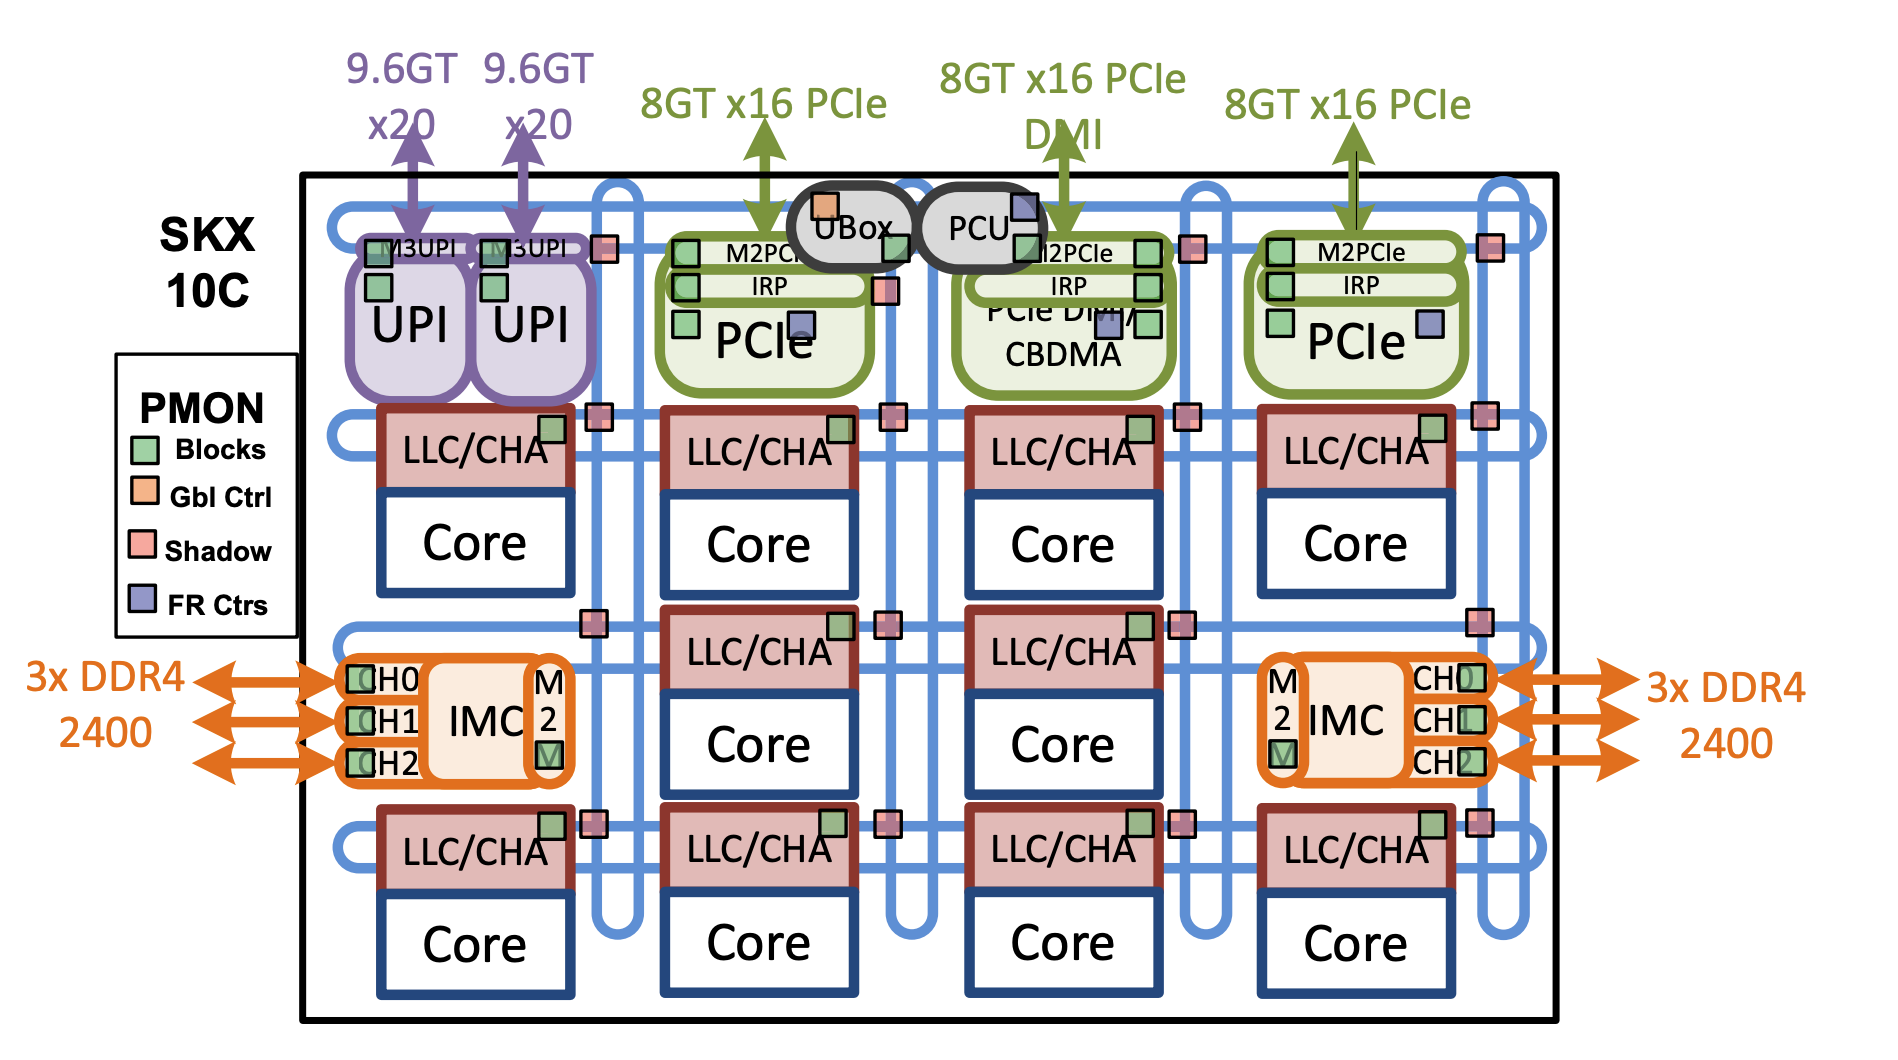
\includegraphics[width=12cm]{images/edl_perf_uncore_intel_skl.png}
    \caption{\label{fig:edl_perf_uncore_intel_skl} Disposition des PMU uncore sur les processeurs Xeon Skylake. \protect\footnotemark}
    \end{figure}
    \footnotetext{source: Intel Xeon Processor Scalable Memory Family Uncore Performance Monitoring Reference Manual.}



    
    
    \paragraph{Rappel PCI.} 
    Le bus PCI a été défini pour établir un bus local de haute performance et de faible coût. Le composant bus PCI et l'interface de carte d'extension sont indépendants du processeur, ce qui permet une transition efficace vers les futurs processeurs, ainsi qu'une utilisation avec des architectures multiprocesseurs. 
    
    

PCI Express a introduit une nouvelle façon d'accéder à l'espace de configuration PCI, où il s'agit simplement d'une cartographie mémoire et où aucun port d'E/S n'est utilisé. 

La spécification PCI définit l'organisation des registres Configuration Space de 256 octets 



Traduit avec www.DeepL.com/Translator
    
    
    Pour identifier les différents matériels PCI, la notation BDF est utilisée: \verb| Bus:Device:Function|. Cela permet d'avoir jusqu'à 256 bus, chacun avec jusqu'à 32 appareils, chacun supportant huit fonctions. Chaque fonction de l'appareil sur le bus dispose d'un espace de configuration de 256 octets et impose une structure spécifique. Tous les périphériques compatibles PCI doivent prendre en charge les champs Vendor ID, Device ID, Command and Status, Revision ID, Class Code et Header Type. Par exemple, le matériel construit par le vendeur Intel aura un code 0x8086\footnote{Source: \url{https://pcisig.com/membership/member-companies?combine=Intel}}.
    


    
    The uncore driver is active if a number of uncore files show up in /sys/devices/
    # ls -d /sys/devices/uncore*


    \subsubsection{/sys interface}
    %%%%%%%%%%%%%%%%%%%%%%%%%%%%%%%%%%
    L'interface Linux \textit{/sys} est un système de fichier virtuel introduit avec la version 2.6 du noyau Linux. Il permet de présenter les différents \textit{devices} du noyau à l'espace utilisateur. Un \textit{device} peut être un matériel, un driver, un bus... Chaque répertoire représente un matériel, et les fichiers s'y trouvant comporte l'information correspondant à son nom (vendeur, évenement. Les matériels peuvent être représentés par bus, grâce au chemin \verb|/sys/bus| comme présenté dans la \autoref{fig:edl_perf_sys_pci}. Pour accéder aux PMU \textit{uncore}, le driver doit être activé. Il est possible de le vérifier enregardant si plusieurs fichier nommés \textit{uncore*} apparaissent dans le dossier \verb|/sys/devices/|. Il est ensuite possible de programmer les PMU grâce à des lectures/écritures dans le fichier \textit{config} correspondant au bon matériel. L'exemple suivant permet d'activer les compteurs \textit{FFC}:
   
    
\begin{lstlisting}[
basicstyle={\scriptsize\ttfamily},
identifierstyle={\color{black}},
language={c},
tabsize=2,
numbersep=8pt,
frame=tlbr,framesep=2pt,framerule=0pt,
morekeywords ={class,run},
]
pci_fd = open("/sys/devices/pci0000:3a/0000:3a:0a.6/config",O_RDWR);
ctl = 0x10100UL; // enable + freeze
pwrite (pci_fd, &ctl, sizeof(ctl), BOX_CTL);
\end{lstlisting}

    
    \begin{figure}
    \center
    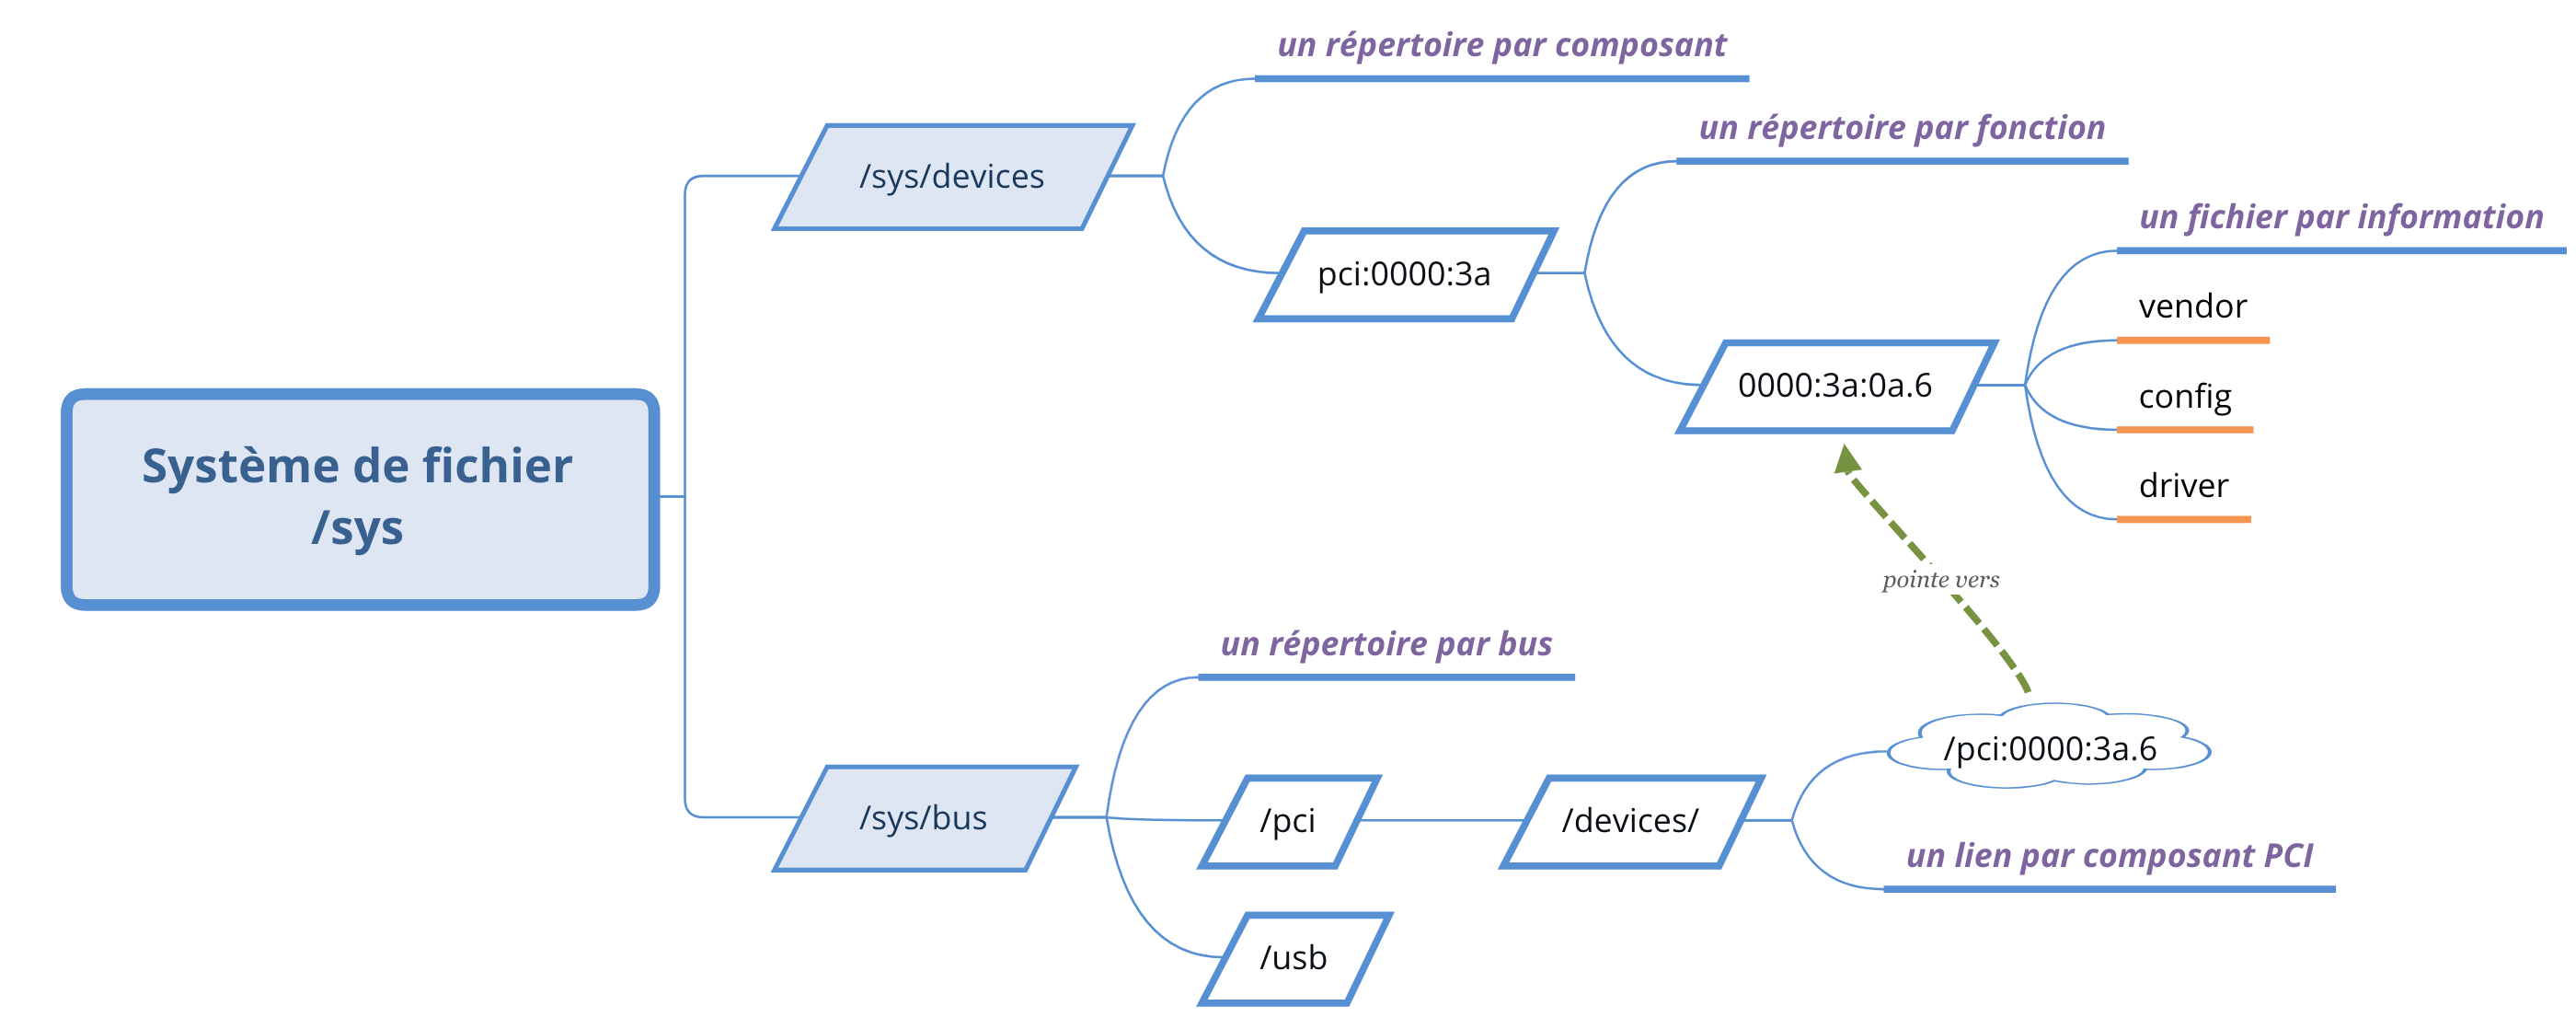
\includegraphics[width=12cm]{images/edl_perf_sys_pci.png}
    \caption{\label{fig:edl_perf_sys_pci} Système de fichier virtuel présentant les matériels PCI.}
    \end{figure}

    
    \subsubsection{lspci + setpci}
    %%%%%%%%%%%%%%%%%%%%%%%%%%%%%%%%%%
    
    Pour interagir avec le matériel PCI, Linux propose deux commandes: \verb|lspci| pour les lister et \verb|setpci| pour les configurer. Cette section présente un exemple de configuration des compteurs permettant de suivre le trafic du bus mémoire d'une architecture Skylake. 
    
    
    
    Comme le montre la \autoref{fig:edl_perf_sys_pci}, les processeurs Xeon Skylake possède deux contrôleurs mémoire (IMC) possédant chacun 3 canaux, pour un total de 6 canaux mémoire. Pour pouvoir configurer ces compteurs, il faut alors obtenir les informations suivantes: identifiant du bus, identifiant du matériel et la fonction. Ces informations peuvent être retrouvée dans la section 1.8.2 de la documentation Intel \cite{Intel2017b}: Identifiant (\verb|0x2042|, \verb|0x2046| et \verb|0x204A|) ainsi que le bus  (2). Pour pouvoir utiliser la notation BDF, il faut alors connaître l'adresse allouée au bus numéro 2 en consultant le registre \verb|0x300| qui stocke l'adresse des différents bus pci pour chaque processeur. La commande \verb|#rdmsr 0x300| renvoie la valeur \verb|800000005d3a1700| et permet de déduire que l'adresse du deuxième bus est \verb|0x3a|. La commande \verb|lspci| permet de s'assurer que les contrôleurs sont bien reconnus et accessibles:
\begin{verbatim}
lspci | grep "3a"                      //Sélectionner le bus correspondant au CPU étudié
      | grep -i "\(2042\|2046\|204A\)" //N'afficher que les controleur mémoires
3a:0a.2 System Intel 2042 
3a:0a.6 System Intel 2046 
3a:0b.2 System Intel 204a 
3a:0c.2 System Intel 2042
3a:0c.6 System Intel 2046 
3a:0d.2 System Intel 204a
\end{verbatim}
    
    À l'aide de la documentation Intel \cite{Intel2017b}, il est ensuite possible de configurer les compteurs de chaque canal mémoire grâce au code présenté dans l'\autoref{lst:edl_perf_setpci}. Les évènements comptés sont construit à partir du tableau 2-108. Le démarrage, l'arrêt et la lecture des compteurs est réalisé de la même façon et peut être consulté sur notre dépôt GitHub\footnote{\url{https://github.com/PourroyJean/performance_modelisation/blob/master/src/tool_PMU/pmu_uncore.sh}}. 

\begin{minipage}{\linewidth}
\begin{lstlisting}[
label=lst:edl_perf_setpci,
basicstyle={\scriptsize\ttfamily},
identifierstyle={\color{black}},
language={bash},
tabsize=2,
numbersep=8pt,
frame=tlbr,framesep=2pt,framerule=0pt,
morekeywords ={class,run},
caption=Configurer les compteurs \textit{uncore} à l'aide de la commande \textit{setpci}.
]
 Channels=(0 1 2 3 4 5)
      bus=3a
  devices=(0a  0a  0b  0c  0c  0d)
functions=( 2   6   2   2   6   2)

for CHAN in $mychannels ;
    #       FREEZE and RESET
    setpci -s ${BUS}:${devices[CHAN]}.${functions[CHAN]} ${pmonunitctrl_hi}=0x1        
    setpci -s ${BUS}:${devices[CHAN]}.${functions[CHAN]} ${pmonunitctrl_lo}=0x2
    #       ZERO the counter:        
    setpci -s ${BUS}:${devices[CHAN]}.${functions[CHAN]} ${pmoncntrupper1_0}=0x0  
    #       RESET MONITORING CTRL REGISTERS        
    setpci -s ${BUS}:${devices[CHAN]}.${functions[CHAN]} ${pmonunitctrl_lo}=0x1
    #       CONFIGURE COUNTER #0 FOR CAS_COUNT.RD and #1 for CAS_COUNT_WR        
    setpci -s ${BUS}:${devices[CHAN]}.${functions[CHAN]} ${pmoncntrcfg_0}=${ev_read}        
    setpci -s ${BUS}:${devices[CHAN]}.${functions[CHAN]} ${pmoncntrcfg_1}=${ev_write}
    #       RELEASE COUNTERS        
    setpci -s ${BUS}:${devices[CHAN]}.${functions[CHAN]} ${pmonunitctrl_hi}=0x0done
\end{lstlisting}
\end{minipage}
    
    
    
    
    \subsubsection{Mapper l'espace d'adressage PCI}
    %%%%%%%%%%%%%%%%%%%%%%%%%%%%%%%%%%
    La deuxième façon d'accéder au compteurs \textit{uncore} est de \textit{mapper} l'esapce d'adressage PCI dans l'espace utilisateur. Les outils développés chez HPE par Frederic Ciesielski,  utilisent principalement cette technique. La première étape est d'obtenir l'adresse du début de cet espace de configuration en utilisant la commande suivante:
\begin{verbatim}
#cat /proc/iomem | grep MMCONFIG  
80000000--8fffffff : PCI MMCONFIG
\end{verbatim}
    Il est ensuite possible de mapper cet espace mémoire dans l'espace utilisateur. En langage C le code présenté dans l'\autoref{lst:edl_perf_mmap} permet de réaliser la configuration des compteurs comme dans l'exemple précédemment réalisé avec \verb|setpci|.
    \begin{lstlisting}[
label=lst:edl_perf_mmap,
basicstyle={\scriptsize\ttfamily},
identifierstyle={\color{black}},
language={c},
tabsize=2,
numbersep=8pt,
frame=tlbr,framesep=2pt,framerule=0pt,
morekeywords ={class,run},
]
mymapping =  mmap(0,0x10000000, 
		            PROT_READ | PROT_WRITE, MAP_SHARED, 		 
		            /dev/mem, 80000000);
for(chan=0;chan<nchan;chan++) { //Pour les 6 canaux memoire 
// FREEZE COUNTERS 
PCIDATA8(bus,chan_dev[chan],chan_func[chan],_Config_add_)=0x1; 
// READ COUNTER 
val0 = (PCIDATA32(bus,chan_dev[chan],chan_func[chan], _PMC0_1) & 0x0000ffff )<<32; 
val0|=  PCIDATA32(bus,chan_dev[chan],chan_func[chan], _PMC0_0); 
// ZERO COUNTERS 
PCIDATA32(bus,chan_dev[chan],chan_func[chan], PMC0_1)=0x0;
PCIDATA32(bus,chan_dev[chan],chan_func[chan], PMC0_0)=0x0;
\end{lstlisting}
    
    
    \subsection{Listes des outils}
    
    - Perf
    http://www.brendangregg.com/perf.html
        
    The perf tool offers a rich set of commands to collect and analyze performance and trace data. The command line usage is reminiscent of git in that there is a generic tool, perf, which implements a set of commands: stat, record, report, [...]
       
        perf is based on the perf_event_open system call and hardware dependent code is developed by Linux kernel developers for supporting various models. It is a very complex tool designed to be used by end users. The only provided interface is the command line, no API is provided. As a consequence, compared to numap, it is impossible to build programming model aware profilers on top of perf.
      
      https://perf.wiki.kernel.org/index.php/Tutorial

        
        
        
    
     

\subsection{Conclusion}   
%%%%%%%%%%%%%%%%%%%%%%%%%%%%%%%%%%
    
    \subsubsection{Recap}
    -	Informations : Pour pouvoir lire les MSR directement, il faut connaître leur adresse, leur masque, comment les initialiser… Ce travail est conséquent car ces informations se trouvent dans la documentation Intel qui fait plusieurs milliers de pages. Aussi, les descriptions de ces événements ne sont pas tout le temps clair, et trouver le bon évènement est complexe. Pour donner un ordre d’idée, le tableau répertoriant les .
    
    Plainte ici 
    https://software.intel.com/en-us/forums/software-tuning-performance-optimization-platform-monitoring/topic/804140
    
    
    -	Droits : De plus, les MSR des dernières architectures Skylake ne sont pas dans les dernières documentation public Intel. Bien qu’à HPE nous y ayons accès, il serait illégal de développer un outil OpenSource basé sur ces informations. Nous sommes actuellement en contact avec Intel pour en discuter
    
    -	Complexité du code : pour accéder à ces compteurs, il faut développer du code bas niveau, assembleur/c. Ce code varie d’un modèle de processeurs à l’autre (même chez le même vendeur) ce qui le rend peu portable. 
    
    -	Compteurs spécifiques : nous voulons accéder aux compteurs uncore, du controleur mémoire, qui mesurent précisément la bande passante. Ces compteurs, récents, ne sont pas supportés par tous les outils et des travaux ont déjà étaient réalisés pour déduire la bande passante en se basant sur des compteurs plus communs comme le compteur de miss dans le dernier niveau de cache (LLC). Cependant comme décrit dans [Florian, p16] le prefecther anticipe certains miss rendant ce compteur inutilisable. Et nous ne pouvons pas envisager de le désactiver comme ils le font dans leur papier.
    

    \textbf{TODO impact de la mesure} TheOverheadOfProfilingUsingPMUhardwareCounters.pdf
        
    We set out to measure the overhead incurred when profiling with PMU hardware counters. Results show how it can vary in many dimensions – the events selected, their frequencies, the workload, the number of events and in particular, the profiling method. An exact measurement of the hardware (vs. software) overheads would require more detailed instrumentation of the kernel – our results only demonstrate the overheads a performance tuner would see from their perspective.
    
    One of the biggest sources of overheads seems to be multiplexing – users concerned with performance are advised not to use more events than there are hardware counters available, in particular in sampling mode. When multiplexing and with a very demanding set of counters of configurations, overheads can reach as much as 25\% - a number more commonly seen when using software instrumentation to monitor workloads. This result suggests that there still might be room for optimization in the perf subsystem.    
        

        
        
        
        
        
        
        
        
        
        
        
        
        
        Il est important de noter que si l'\textit{hyperthreading} est désactivé, les PMU ne posséderont que la moitié des compteurs disponibles (8) .
        
    \subsubsection{Conclusion}
    %%%%%%%%%%%%%%%%%%%%%%%%%%%%%%%%%%

    La majorité des compteurs n'est donc pas supportée par les constructeurs bien qu'ils soient documentés pour certains d'entre eux. La  principale difficulté pour les programmeurs est donc de trouver ces compteurs, de les utiliser et d'en comprendre la signification. 


\textbf{LIRE RESUME - Hardware Counter}

3.9 Caveats of Hardware Counters

While performance counters are a powerful tool, care must be taken when
using the results.

3.9.1 Accuracy
    Although aggregate event counts are sometimes referred to as “exact counts,” and profiling is statistical in nature, sources of error exist for both modes. As in any physical system, the act of measuring perturbs the phenomenon being measured. The counter interfaces necessarily introduce overhead in the form of extra instructions (including system calls), and the interfaces cause cache pollution that can change the cache and memory behavior of the monitored application. The cost of processing counter overflow interrupts can be a significant source of overhead in sampling-based profiling. Furthermore, a lack of hardware support for precisely identifying an event’s address may result in incorrect attribution of events to instructions on modern superscalar, out-of-order processors, thereby making profiling data inaccurate. Hardware designers use performance counters for internal testing, and they publish their use mainly as a courtesy. When asked they will admit that very little testing goes into the counters, and that caution should be exercised when using any counter (though commonly used ones such as retired instructions or cycle count can generally be counted on to be reliable). Before using an event, it is a good idea to read the documentation for your chip and check the vendor supplied errata to make sure there are no known problems with the event. Also a few sanity checks should be run on small programs to make sure the results are what you expect. Modern chips have advanced features that can cause unexpected results, such as hardware prefetchers that can vastly change cache behavior compared to a traditional view of how caches behave. Another issue to worry about is multiplexing. When enough counters are not available, the operating system might multiplex the counters. This adds a certain amount of inaccuracy to returned results.

3.9.2 Overhead
    Even though performance counters have relatively low overhead, the overhead is enough that it can be measured. On a counter overflow an interrupt 48 Performance Tuning of Scientific Applications routine interrupts program flow, which can cause timing (and even cache) behavior changes that would not happen if counters were not being used. Also, libraries such as PAPI add a certain amount of overhead each time a routine is called, which can show up in counter results. 3.9.3 Determinism It is often expected that if the same program is run twice, the resulting performance results should be the same between runs. Even if a program is specifically set up to be deterministic, various factors can cause different counts [356]. The operating system can put parts of the program in different parts of memory run-to-run (address space randomization, a security feature of Linux that can be disabled). Some counts can vary due to operating system conditions and other programs running on the system. Branch prediction and cache rates can be affected by the behavior of other programs and by the operating system accessing memory. Especially on x86, some counters increment whenever a hardware interrupt happens, which can artificially increase counts. These determinism problems are magnified on multi-core workloads, as the different interacting threads are scheduled in a non-deterministic fashion.

3.10 Summary
    Hardware performance counters are a powerful tool that can offer insight into the underlying system behavior. As machines become more complex, interactions between applications and systems become non-intuitive and harder to understand. This is compounded by the move to large massively parallel systems. The use of performance counters and tools such as PAPI can greatly increase understanding and enable performance improvements of difficult codes

 
%%%%%%%%%%%%%%%%%%%%%%%%%%%%%%%%%%%%%%%%%%%%%%%%%%%%%%%%%%%%%%%%%%%%%%%%%%%%%%%%%%%%%%%%%%%%%%%%%%%%%%%%%%%%%%%%%%%%%%%%%%%%%%%%%%%%%%%%%%%%%%%%%%%%%%%%%%%%%%%%%%%%%%%%%%%%%%%%%%%%%%%%%%%%%%%%%%%%%%%%%
\subsection{Analyse de performances}%%%%%%%%%%%%%%%%%%%%%%%%%%%%%%%%%%%%%%%%%%%%%%%%%%%%%%%%%%%%%%%%%%%%%%%%%%%%%%%%%%%%%%%%%%%%%%%%%%%%%%%%%%%%%%%%%%%%%%%%%%%%%%%%%%%%%%%%%%%%%%%%%%%%%%%%%%%%%%%%%%%%%%%%%%%%%%%%%%%%%%%%%%%%%%%%%%%%%%%%%



%%%%%%%%%%%%%%%%%%%%%%%%%%%%%%%%%%%%%%%%%%%%%%%%%%%%%%%%%%%%%%%%%%%%%%%%%%%%%%%%%%%%%%%%
%%% |   _  \      /  __  \   /  __  \  |   ____|   |  |     |  | |  \ |  | |   ____| %%%
%%% |  |_)  |    |  |  |  | |  |  |  | |  |__      |  |     |  | |   \|  | |  |__    %%%
%%% |      /     |  |  |  | |  |  |  | |   __|     |  |     |  | |  . `  | |   __|   %%%
%%% |  |\  \----.|  `--'  | |  `--'  | |  |        |  `----.|  | |  |\   | |  |____  %%%
%%% | _| `._____| \______/   \______/  |__|        |_______||__| |__| \__| |_______| %%%
%%%%%%%%%%%%%%%%%%%%%%%%%%%%%%%%%%%%%%%%%%%%%%%%%%%%%%%%%%%%%%%%%%%%%%%%%%%%%%%%%%%%%%%%

\subsubsection{Modèle du Roofine} \label{sec:roofline}
%%%%%%%%%%%%%%%%%%%%%%%%%%%%%%%%%%%%%%%%%%%%%%%%%%%%%%%%%%%%%%%%%%%

%%%%%%%%%%%%%%%%%
\paragraph{Motivation et objectifs}
%%%%%%%%%%%%%%%%%
Présenté par William et al. en 2009 \cite{Williams2008}, le modèle du \textit{roofine} est un modèle de performance simple qui représente graphiquement les performances d’un code en situant sa performance par rapport au performances maximales de l’architecture. L’objectif principale de ce modèle est de donner le pourcentage de la performance disponible atteinte par un code. L’intérêt de ce model est de restreindre l’analyse de performance aux deux ressources importantes pour les applications HPC: la performance calculatoire (GFLOP/s) et la performance du bus mémoire (GB/s).
Le modèle est utilisé pour représenter les différentes fonctions clefs d’une application. Ainsi, le programmeur pourra commencer son travail d’optimisation sur les fonctions avec le plus de potentiel.

\begin{figure}
    \center
    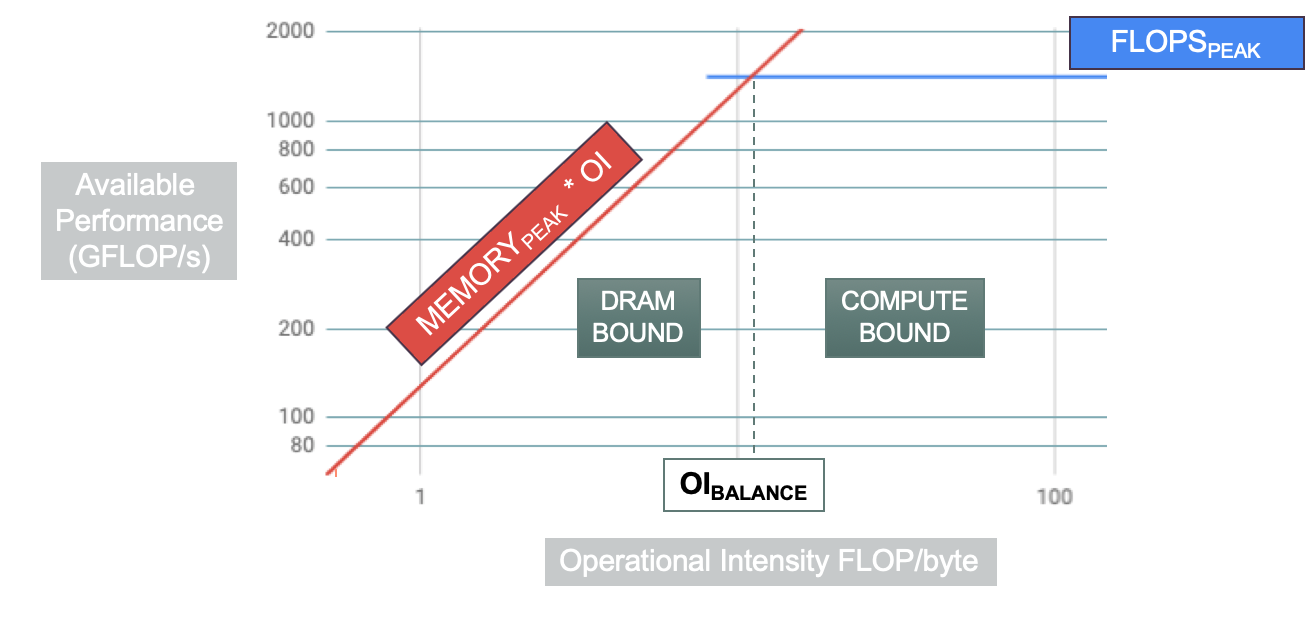
\includegraphics[width=10cm]{images/roofline.png}
    \caption{\label{fig:roofline} Représentation graphique du modèle du \textit{roofline}. En fonction de son l'intensité opérationnelle, la performance d'un code sera limitée par la bande passante ou par le processeur.}
\end{figure}


La \autoref{fig:roofline} montre une représentation du modèle du \textit{roofine}. Sur l’axe des abscisse est représentée l’intensité opérationnelle de l’algorithme (en flops/byte) qui correspond nombre d’opération flottante appliqué à chaque byte de donnée amené depuis la mémoire. Sur l’axe des ordonnées est représentée la performance de calcul mesurée en GFLOP/s.
Chaque hot spot sont placés en fonction de leur intensité opérationnelle, calculée à partir de la lecture du code, et de sa performance, mesurée lors de l’exécution.

%%%%%%%%%%%%%%%%%
\paragraph{Preuve et construction}
%%%%%%%%%%%%%%%%%
L’objectif du modèle est de déterminer si la performance du code pour une architecture donnée est structurellement limité par la performance du processeur ($FLOPS_{peak}$ en $GFLOP/s$) ou bien par la performance du bus mémoire ($MEMORY_{peak}$ en $GB/s$). Une application réalisant la lecture de deux nombres pour y réaliser des centaines d’opérations verra ses performances limitées par la capacité de calcul $FLOPS_{peak}$ du processeur. Inversement, une application devant lire un grand jeu de données pour ne réaliser qu'une opération sur chaque valeur, verra ses performance limitées par celle du bus mémoire $MEMORY_{peak}$. On peut estimer la quantité de calculs à réaliser sur chaque donnée en calculant son Intensité Opérationnelle  ($\text{OI}$ en $flop/byte$). Pour cela il faut lire le code source pour compter manuellement le nombre d’opérations réalisées ($\text{\#FLOP}$) et le nombre de données nécessaires chargées depuis la mémoire ($\text{\#BYTE}$). On peut ainsi calculer l’Intensité Opérationnelle d’un code en faisant le ratio des deux valeurs.

\begin{equation}
\begin{aligned}
        \text{OI}_{kernel} =\ &\cfrac{\text{\#FLOP}}{\text{\#BYTE}}
\end{aligned}
\end{equation}

Le temps pour exécuter le code ($\text{TEMPS}_{theorique}$), sera le temps mis par la ressource la plus utilisée par le code. On peut estimer ce temps par la formule suivante.
\begin{equation}
\begin{aligned}
     \text{TEMPS}_{theorique} =\  &max 
     \begin{cases} 
        \quad \cfrac{\text{\#FLOP}}{\text{FLOPS}_{peak}}    \\[15pt]
        \quad \cfrac{\text{\#BYTE}}{\text{MEMORY}_{peak}}
    \end{cases}
\end{aligned}
\end{equation}




La performance théorique du code ($\text{PERF}_{theorique}$ en GFLOP/s) peut être calculée grâce aux transformations successives de l'\autoref{eq:PERFT}.
\begin{equation}
\begin{aligned}
\label{eq:PERFT}
\cfrac{\text{TEMPS}_{theorique}}{\text{\#FLOP}}  =\ &\text{max}
\begin{cases} 
    \cfrac {1}{\text{FLOPS\_{peak}}}    \\[15pt]  
    \cfrac {\cfrac{\text{\#BYTE}}{\text{MEMORY}_{peak}}}{\text{\#FLOP}} 
\end{cases}\\[20pt]
\cfrac{\text{\#FLOP}}{\text{TEMPS}_{theorique}}  =\ &\text{min}
\begin{cases} 
    \text{FLOPS}_{peak}    \\[15pt]  
    \cfrac{\text{\#FLOP}}{\text{\#BYTE}} \times \text{MEMORY}_{peak}
\end{cases}\\[20pt]
\text{PERF}_{theorique}  =\ &\text{min}
\begin{cases} 
    \text{FLOPS}_{peak}    \\[15pt]  
    \text{OI}_{kernel} \times \text{MEMORY}_{peak} 
\end{cases}
\end{aligned}
\end{equation}



Pour une architecture, il faut déterminer pour quelle intensité opérationnelle une application est limitée par la mémoire ou le processeur. Pour cela, il faut calculer l’intensité opérationnelle ($\text{OI}_{balance}$) correspondant au croisement des deux droites sur la \autoref{fig:roofline}. 

\begin{equation}
\begin{aligned}
 \text{FLOPS}_{peak} =\ &\text{OI}_{balance} \times \text{MEMORY}_{peak} \\[20pt]
 \text{OI}_{balance} =\ &\frac{\text{MEMORY}_{peak}} {\text{FLOPS}_{peak}} 
\end{aligned}
\end{equation}

Une application dont l’intensité opérationnelle est inférieure à $\text{OI}_{balance}$ verra sa performance limitée par le système mémoire. Plus rarement, si l’intensité opérationnelle d’une application est supérieure à $\text{OI}_{balance}$, la performance sera alors limitée par le processeur.

\paragraph{Construction}
La première étape dans la construction du graphique est de tracer les deux axes limitant les performances d’un code. Ces deux droites représentes les performances crêtes de la mémoire et du processeur. Pour obtenir ces valeurs, elles peuvent être calculées à partir des spécifications du processeurs. Cependant, avec la complexification des architectures, il est difficile de les atteindre même avec des benchmarks prévus à cet effet. Il est donc préférable de les représenter par des valeurs mesurées comme indiqué dans la littérature  \cite{farjallah2014preparing}. Pour la mémoire le benchmark Stream peut être utilisé. Pour la performance du processeur, nous utilisons le générateur de benchmark présenté dans la \autoref{sec:kg}. D’autres travaux sont venus compléter les benchmarks disponibles pour caractériser l’architecture \cite{lo2014roofline}.




%%%%%%%%%%%%%%%%%
\paragraph{Évolutions}
%%%%%%%%%%%%%%%%%


Le \textit{roofine} a reçu de nombreuse améliorations depuis sa création. En 2014, les travaux \cite{Ilic2014} constate que le modèle originale n’est pas suffisament précis à cause de la faible précision de caractérisation de l’architecture. En effet, un code pouvant profiter de la localité des données dans les caches pourrait atteindre des performances supérieur au maximum prévu par le modèle utilisant seulement le bande passante mémoire. Inversement, la performance crête est calculé pour un code utilisant tous les coeurs du processeur, avec des instructions FMA vectorisées. Cependant, par leur nature, certain code ne peuvent pas utiliser ces  caractéristiques. La performance crête étant alors impossible à atteindre. Le modèle Cache-Aware Roofline Model (CARM) \cite{Ilic2014} a ainsi été développé permettant de représenter la performance des différents niveaux de caches. Cependant, le programmeur doit comprendre si son application peut tirer partie de cette localité, ce qui peut rendre cette approche plus difficile. Le modèle à depuis été affiné avec le Locality Aware Roofline Model (LARM) \cite{Denoyelle2018} permettant de modéliser les accès en mémoire non uniforme (NUMA).
D’autres travaux essaient d’automatiser sa construction \cite{lo2014roofline} pour faciliter son usage. L’outil de profiling d’Intel a intégré les modèles CARM et LARM pour automatiser la recherche des hot spot et afficher leur performance sur un même graphique. Pour cela, il désassemble le code et calcule l’intensité opérationnelle de la boucle étudiée.


%%%%%%%%%%%%%%%%%
\paragraph{Critiques}
%%%%%%%%%%%%%%%%%

La force de cette approche est de montrer rapidement au programmeur si son application est efficace ou non. Dans le cas échéant, il sait s’il doit travailler sur l’optimisation des flops ou de la mémoire. En modélisant les principaux kernels de son application, le programmeur saura sur lesquels ses optimisations seront le plus bénéfiques.

Bien d’ayant reçu de nombreuses améliorations, ce modèle doit être utilisé pour commencer l’analyse de performance. Mais il ne permet pas de modéliser n’y de comprendre finement la raison d’une performance.
La majorité des applications étant limitée par la bande passante mémoire, il est rare d’utiliser ce modèle pour modéliser la performances des unités de calculs. Mais il peut être intéressant de calculer l’intensité opérationnelle d’une boucle pour s’en assurer avant d’apporter des optimisations. De plus, les accélérateurs à venir essaient de réduire le trou de performance entre les processeurs et la mémoire. Cette modélisation est donc importante pour l’analyse de performance.


\newpage

\section{Caractérisation des architectures}\label{sec:caracterisation}


\textbf{TODO}
- lecture thèse - 1 Décomposition automatique des programmes parallèles pour l’optimisation et la prédiction de performance. Mihail Popov\\




%%%%%%%%%%%%%%%%%%%%%%%%%%%%%%%%%
\subsection{Benchmarks}
%%%%%%%%%%%%%%%%%%%%%%%%%%%%%%%%%

En informatique, un benchmark est un code, ou un ensemble de code, permettant de mesurer la performance d'une solution et d'en vérifier ses fonctionnalités. Les benchmarks peuvent être utilisés pour plusieurs raisons, énumérée dans le paragraphe suivant. 

% UTILITE
\paragraph{Utilité des benchmarks.}
Dans le domaine du HPC, les benchmarks sont utilisés pour raisons différentes. 
    
    De nombreuses architectures sont présentés chaque années, avec chacune des caractéristiques différentes. Pour connaître leur potentiel, des codes de références sont utilisés pour apprécier leur performances pour un certain types d'application. 
    
    Les benchmarks peuvent aussi être utilisés lors de la phase de conception d'une architecture. Cela permet d'estimer la futur performance d'un matériel avant qu'il ne soit produit (grâce à des simulateurs par exemple). Les benchmarks utilisés peuvent avoir les mêmes profils que les applications qui seront réellement exécutées sur le supercalculateur en production. Cela permet à l'industriel qui le produit de la placer sur des domaines sur lesquels il performe particulièrement.
     
    
    Utiliser un benchmark évite à l'acheteur de fournir des codes et des données (souvent sensibles) pour la conception d'une plate-forme. En utilisant un benchmark, il est facile pour un concepteur de cluster de tester différentes configuration sur des processeurs différents, avec des tailles de mémoires plus ou moins grandes et des réseaux de vitesses différentes. 
    Les codes de benchmark sont plus la majorité en version libre de droit. Cela permet leur large utilisation et permet de comparer la performance de différentes plate-formes. Le TOP500 réalisé grâce au benchmark HPL en est un exemple.
     
    
    Aussi, les centres de données sont des zones très sensibles. Il arrive que les ingénieurs ayant construit le supercalculateur n'y ai même plus accès une fois ce dernier installé. En utilisant des benchmarks libre de droit, l'utilisateur peur l'exécuter et renvoyer le profil extrait pour permettre aux architectes d'en comprendre les performances. L'utilisation de benchmark dont le code est souvent beaucoup plus simple que celui des applications réelles permet de rapidement identifier des problèmes de performances. 
    
    La complexité des architectures rend difficile la prédiction de la performance d'une plate-forme par la simple lecture de ses caractéristiques techniques ($PERFORMANCE_{crête}$). Il est donc nécessaire d'utiliser une application pour en mesurer la performance maximale atteignable ($PERFORMANCE_{max}$). Le classement du TOp500 fournit ces informations et on constate de grand écart entre ces deux performance pouvant être de plus de 50\%. Le code des benchmarks étant plus simple que celui des applications, un utilisateur voulant atteindre la performance maximale avec son application pourra regarder comment le benchmark a été codé. 


\paragraph{Trois types de benchmarks} Il existe différents types de benchmarks qui peuvent être classés en trois familles \cite{Staelin2004}: les benchmarks, les benchmarks noyaux et les micro-benchmarks.
    
    Les benchmark sont des applications complètes exécutant différent types d'instructions: calculs, transferts mémoire, réseaux... Il peut aussi arriver que des applications réelles soient finalement utilisées comme programme de benchmark tel que BSMBnech \cite{HPC:bsmbench} utilisé pour réaliser des motifs de calculs similaires à ceux de en théorie de jauge sur réseau (physique des particules).
    
    La deuxième famille de benchmarks regroupe les benchmarks noyaux. Ces codes sont généralement extraits d'un application et sont donc plus petits. Les deux benchmark les plus connus sont HPL \cite{HPC:hpl} et STREAM \cite{HPC:stream}. Le benchmark STREAM conciste en l'exécution de quatre fonctions différentes très utilisés dans les application HPC. A l'origine utilisée pour étudier les différences de performances entre deux architectures pour exécuter des applications pour la modélisation du climat, ce code est aujourd'hui très utiliser pour mesurer la bande passante mémoire atteignable sur un bus mémoire. 
   
    Enfin, les micro-benchmark sont des benchmark noyaux qui permettent un d’isoler la partie de l’architecture à stresser. Plus simples, ils permettent de tirer des conclusion sur la performance du matériel. Cela permet d’être sur que l’on mesure bien ce que l’on souhaite et que la performance mesurée n’est pas influé par une autre partie.
    Par exemple, lmbench \cite{HPC:lmbench} est une suite de benchmarks portables utilisés pour mesurer des caractéristiques importantes de la mémoire telles que la bande passante, la latence mémoire et les performances des différents niveaux de cache.
    On peut également citer les travaux \cite{Saavedra1995, gonzalez2010servet} pour la caractérisation des différents niveaux de la hiérarchie mémoire. Les informations récupérées permettent ensuite d'implémenter des optimisations telles que le le \textit{loop tiling} pour s'adapter parfaitement aux différents niveaux de caches.



\paragraph{Construction d'un benchmark} Pour construire un benchmark, deux méthodes peuvent être utilsées. 
    La première est de l'écrire en s'inspirant d'une application réelle ou en implémentant des fonctions pour \textit{stresser} certaines parties de la plate-forme.
    La deuxième méthode est de générer un code de benchmark grâce à un premier code générateur. La génération a l'avantage de faciliter le test de plusieurs configurations différentes en faisant varier les paramètres d'entrée, la taille des jeux de données, ou encore l'algorithme utilisé pour résoudre une tâche. Ainsi, le logiciel de GeneNetWeaver \cite{schaffter2011genenetweaver} peut être utilisé pour générer dynamiquement des modèles génétiques pouvant ensuite eux même être utilisés comme benchmark. Le Benchmark Generator (BM) \cite{younes2003benchmark} peut lui être utilisé pour résoudre dynamiquent le problème du \textit{voyageur de commerce}.


\subsubsection{Les benchmark de processeur}
%%%%%%%%%%%%%%%%%%%%%%%%%%%%%%%%%


\paragraph{HGEMM}






\paragraph{HPL} Les premières versions du benchmark remonte aux années 1979. Le benchmark LINPACK était alors utilisé pour estimer le temps de résolution d'un problème d'algèbre. Ce programme utilisait alors une bibliothèque mathématiques du même nom \textit{LINPACK}. Son utilisation comme benchmark est plus un accident qu'une réelle volonté. L'annexe B du manuel de l'utilisateur proposait aux utilisateeurs d'estimer les temps de résolution de leur problème en fonction de la machine utilisée. Pour pouvoir être utilisé sur les supercalculateurs, le benchmark à été parallélisé, changeant ainsi de nom en Highly Parallel Computing Benchmark ou HPLinpack ou encore HPL.  Le benchmark HPL est utilisé pour construire le  classement du \textit{Top500} \cite{HPC:top500}. Il est utilisé pour mesurer le nombre maximum d'opération à virgule flottantes par seconde (FLOPS) qu'un superordinateur est capable de fournir en résolvant un système linéaire d'équations utilisant la décomposition LU. Ainsi, avant d'être un benchmark de processeur, c'est un benchmark de librairie DGEMM (Intel MKL, netlib, GotoBLAS). La force de ce benchmark est de n'avoir qu'un résultat (soit la sommation des puissances de calculs de chaque coeur utilisé). Il est donc très facile de comparer deux clusters. Bien que mondialement utilisé, le HPL à un principale défaut qui est d'estimer la performance d'une plate-forme en ne mesurant que sa capacité de calcul. Cependant, comme nous l'avons montré précédemment, la performance de la majorité des applications est limitée par la performance de la bande passante. La mesure du HPL n'est donc pas la plus représentative de la puissance d'un supercalculateur atteignables par des applications réelles. 




\paragraph{High Performance Conjugate Gradient (HPCG) \cite{Dongarra2013}} 
Admettant la faiblesse du benchmark HPL son concepteur, Jack Dongarra, se mis à la recherche d'un ou d'un ensemble de benchmark permettant de mieux caractériser ces plate-formes. Avec Michael Heroux et Piotr Luszczek ils présenteront alors en 2015 le benchmark HPCG (high performance conjugate gradient). HPCG permet de couvrir de nombreux motifs de communication (globale et voisinage) et de calculs  (mis-à-jour de vecteur, multiplication de matrices creuses). 
Le premier pré-requis étaient alors de pouvoir produire, grâce à ce nouveau benchmark, un classement des supercalculateurs représentatif de leur performance pour exécuter des applications réelles. Le deuxième pré-requis fait suite à la crainte de voir la conception des processeurs adapté à leur performance pour HPL \cite{Dongarra2013}. Ainsi, HPCG utilise une métric qui poussera les concepteurs de processeurs à améliorer leurs matériels pouvant profiter aux applications réelles. Là où HPL ne fournit qu'un seul résultat par exécution, HPCG en présente 128. Le classement du Top500 est aujourd'hui publié avec les valeurs obtenues par HPL et par HPCG\footnote{classement HPCG: \url{https://www.top500.org/hpcg/lists/2018/06/}}. Bien que plus représentatif des applications réelles que le benchmark HPL, il ne couvre qu'un seul type d'application ayant un faible ratio d'accès mémoire par calcul effectué. Cependant, malgré la meilleur adéquation de HPCG pour caractériser les plate-formes, le benchmark HPL sera toujours utilisé. Principalement pour des raisons d'historiques, il permet de suivre l'évolution des architectures depuis plus de 25 ans. 





\paragraph{HPC Challenge (HPCC)} Cette suite de benchmark vient compléter le benchmark HPL avec des 6 codes dont certains réalisant des accès aux données permettant aussi de caractériser le système mémoire (voir \autoref{pic_bench_hpcc}). La suite de benchmark est ainsi composé de HPL, Stream, DGEMM, RandomAccess, b\_eff, PTRANS, FFT. Avec l'ajout de ces six autres codes, la suite HPCC est plus représentative des applications réelles Ces codes existaient avant la création de la suite HPCC. Le travail réalisé a permis de les regrouper dans une même suite, et de les améliorer avec des systèmes de vérifications et de rapport. Une fois compilé, un seul programme exécutable et généré permettant de faciliter son usage avec un gestionnaire de \textit{job}\footnote{\url{http://citeseerx.ist.psu.edu/viewdoc/download?doi=10.1.1.170.1239&rep=rep1&type=pdf}}. Un seul exécutable étant généré, l'environnement d'exécution est le même pour tous les benchmark de la suite (pas d'optimisaion de page large pour un seul benchmark de la suite). 

\begin{figure}
    \center
    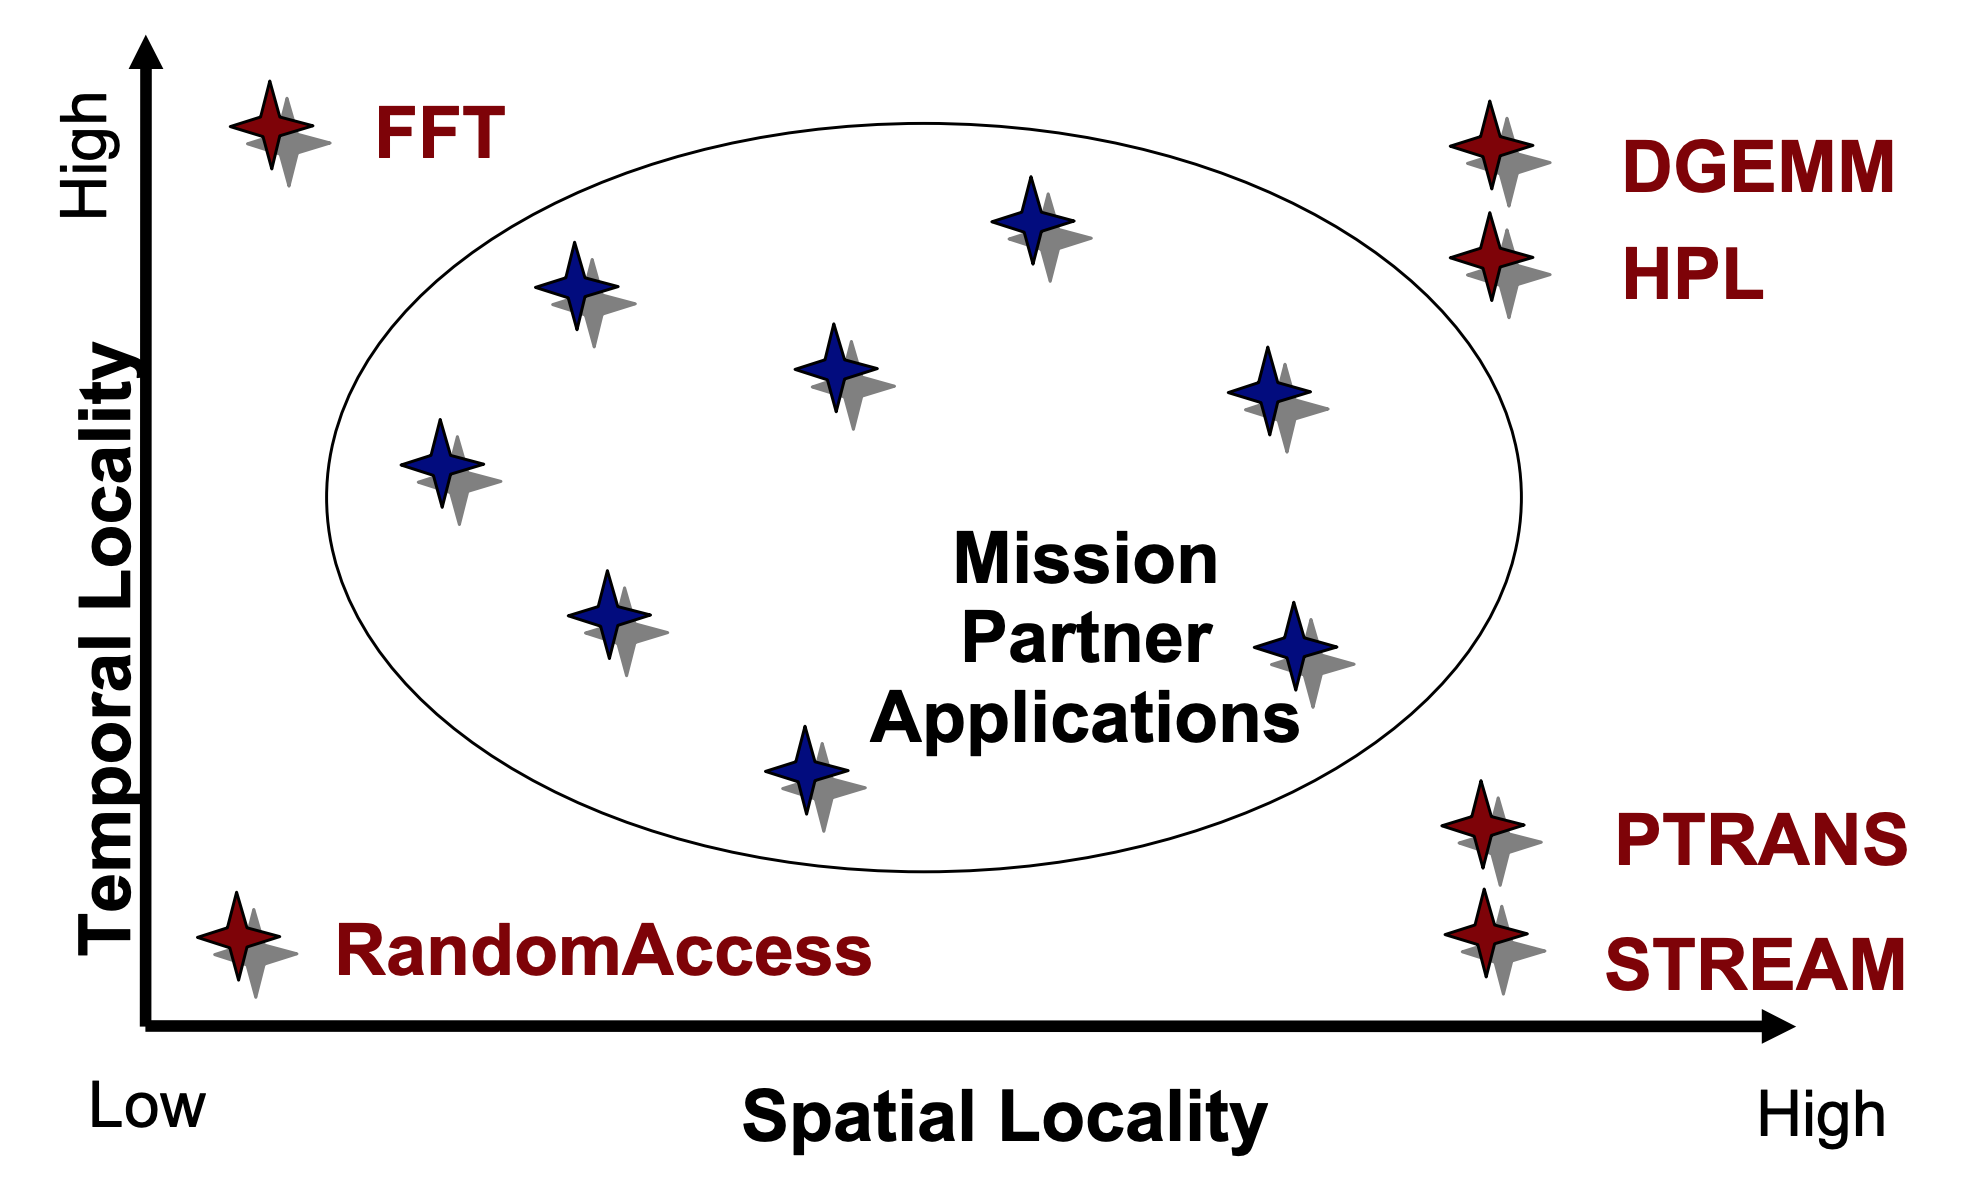
\includegraphics[width=10cm]{images/bench_hpcc.png}
    \caption{ La suite de benchmark HPCC utilise des codes utilisant des localités différentes permettant de mieux caractériser les architectures
    \label{pic_bench_hpcc}}
\end{figure}





\paragraph{NAS Parallel Benchmarks} Ce benchmark développé par la NASA est un ensemble de code permettant d'évaluer la performance de calculs d'un supercalculateur. Le code regroupe cinq kernels et trois petite application dérivé d'application du domaine de la mécanique des fluides. Bien que similaire à HPCG, la différence principale vient de l'initialisation des matrices utilisant une distribution uniforme des données dans chaque ligne. Ce manque de réalisme et la non utilisation de préconditionnement font du benchmark HPCG une meilleure alternative pour ce genre de tests. De plus, les imlémentations des benchmarks divergent entre chaque architecture rendant leur comparaison plus difficile.




\paragraph{SPEC CPU2017} Cette nouvelle génération de benchmark produite par SPEC (Standard Performance Evaluation Corporation) qui fait suite à la version précédente CPEC CPU2006. Ces deux initiatives ont permis de regrouper des applications réelles de tailles différentes mais donc les performances sont limités par la puissance de calcul de l'architecture. Les applications sélectionnés sont facilement portables. La première version contenait deux suites de benchmarks (CINT2006 et CFP2006à permettant demesurer et comparer les performances de calculs en utilisant des opérations entières ou à nombre flottant. L'objectif principale de ce ces codes était alors de caractériser les perofrmance du processeur, de la hiérachie mémoire et du compilateur. La version 2017 possède 43 benchmarks qui sont portées sur plusieurs architectures dont AMD64, Intel IA32, Power ISA ou SPARC. Les benchmarks sont organisés en quatre suites permetant de mesurer le débit et vitesse d'exécution d'opérations utilisant des nombres entiers ou flottant.  Les différents benchmarks ont un domaine d'application spécifique (compression vidéo, rendu 3D...) et peuvent être utilisé pour la conception de processeur optimisés pour ces charges de travail \cite{Panda2018}. Malheureusement le prix de ces benchmarks avoisine les 1000\$. Cependant les nombreux résultats, libres de droits, sont publiés leur site internet. 

\paragraph{SHOC \cite{danalis2010scalable}.} Les plate-formes HPC modernes deviennent toujours plus hétérogènes avec l'utilisation d'accélérateurs comme les GPU ou les DSP. Suite à ce constat, la suite de benchmark Scalable HeterOgeneous Computing (SHOC) a été élaborée pour permettre l'évaluation de la performance et de la montée en charge de tels systèmes. La suite est composée de micro-benchmark et de kernel-benchmark permettant d'évaluer précisément une architecture mais aussi celle d'une plate-forme regroupant plusieurs serveurs grâce à une implémentation MPI. Les codes utilise OpenCL et CUDA pour permettre une large utilisation. Une partie des codes est utiliser pour stresser l'achitecture et identifier des problèmes matériels pouvant impacter la performance: mémoire défaillante ou un mauvais refroidissement. L'autre partie des codes est utilisé pour mesurer la performance de l'architecture grâce à des applications proches de celles utilisés en production. Le code source de la suite de benchmarks est disponible en ligne \footnote{\url{https://github.com/vetter/shoc/wiki}}.


\paragraph{lmbench ici}
In lmbench, McVoy and Staelin replaced array access with
a linked list traversal to allow indirect and randomized access
patterns [7]. This advance was necessitated by improvements
in hardware prefetching

\paragraph{X-Ray \cite{Yotov2004}} Pour aider les programmeurs à écrire de nouveaux benchmarks permettant de mesurer certains paramètres matériel l'outil X-Ray a été mis au point. X-Ray est un framework permettant l'automatisation du développement de benchmark. L'outil est capable de générer plusieurs benchmark dynamiquement en tenant compte de l'exécution des premières versions. Si un benchmark a besoin de connaitre la latence mémoire d'un niveau de cache, X-Ray exécutera alors le benchmark permettant de le calculer avant. X-Ray peut par exemple calculer la fréquence du processeur en ajoutant quatre nombres entiers avec des dépendances pour éviter les optimisations des processeurs superscalaires. Des benchmarks sont aussi disponible pour caractériser la hiérarchie mémoire (associativé, taille des blocs, capacité, latence). Les résultats présentés sont annoncés plus précis que ceux donné par les autres outils de l'état de l'art. Différents tests ont été réalisés sur des ordinateur personnel, des serveurs ou encore des systèmes embarqués. Malheureusement le code n'est plus disponible pour être testé. 

\begin{figure}
    \center
    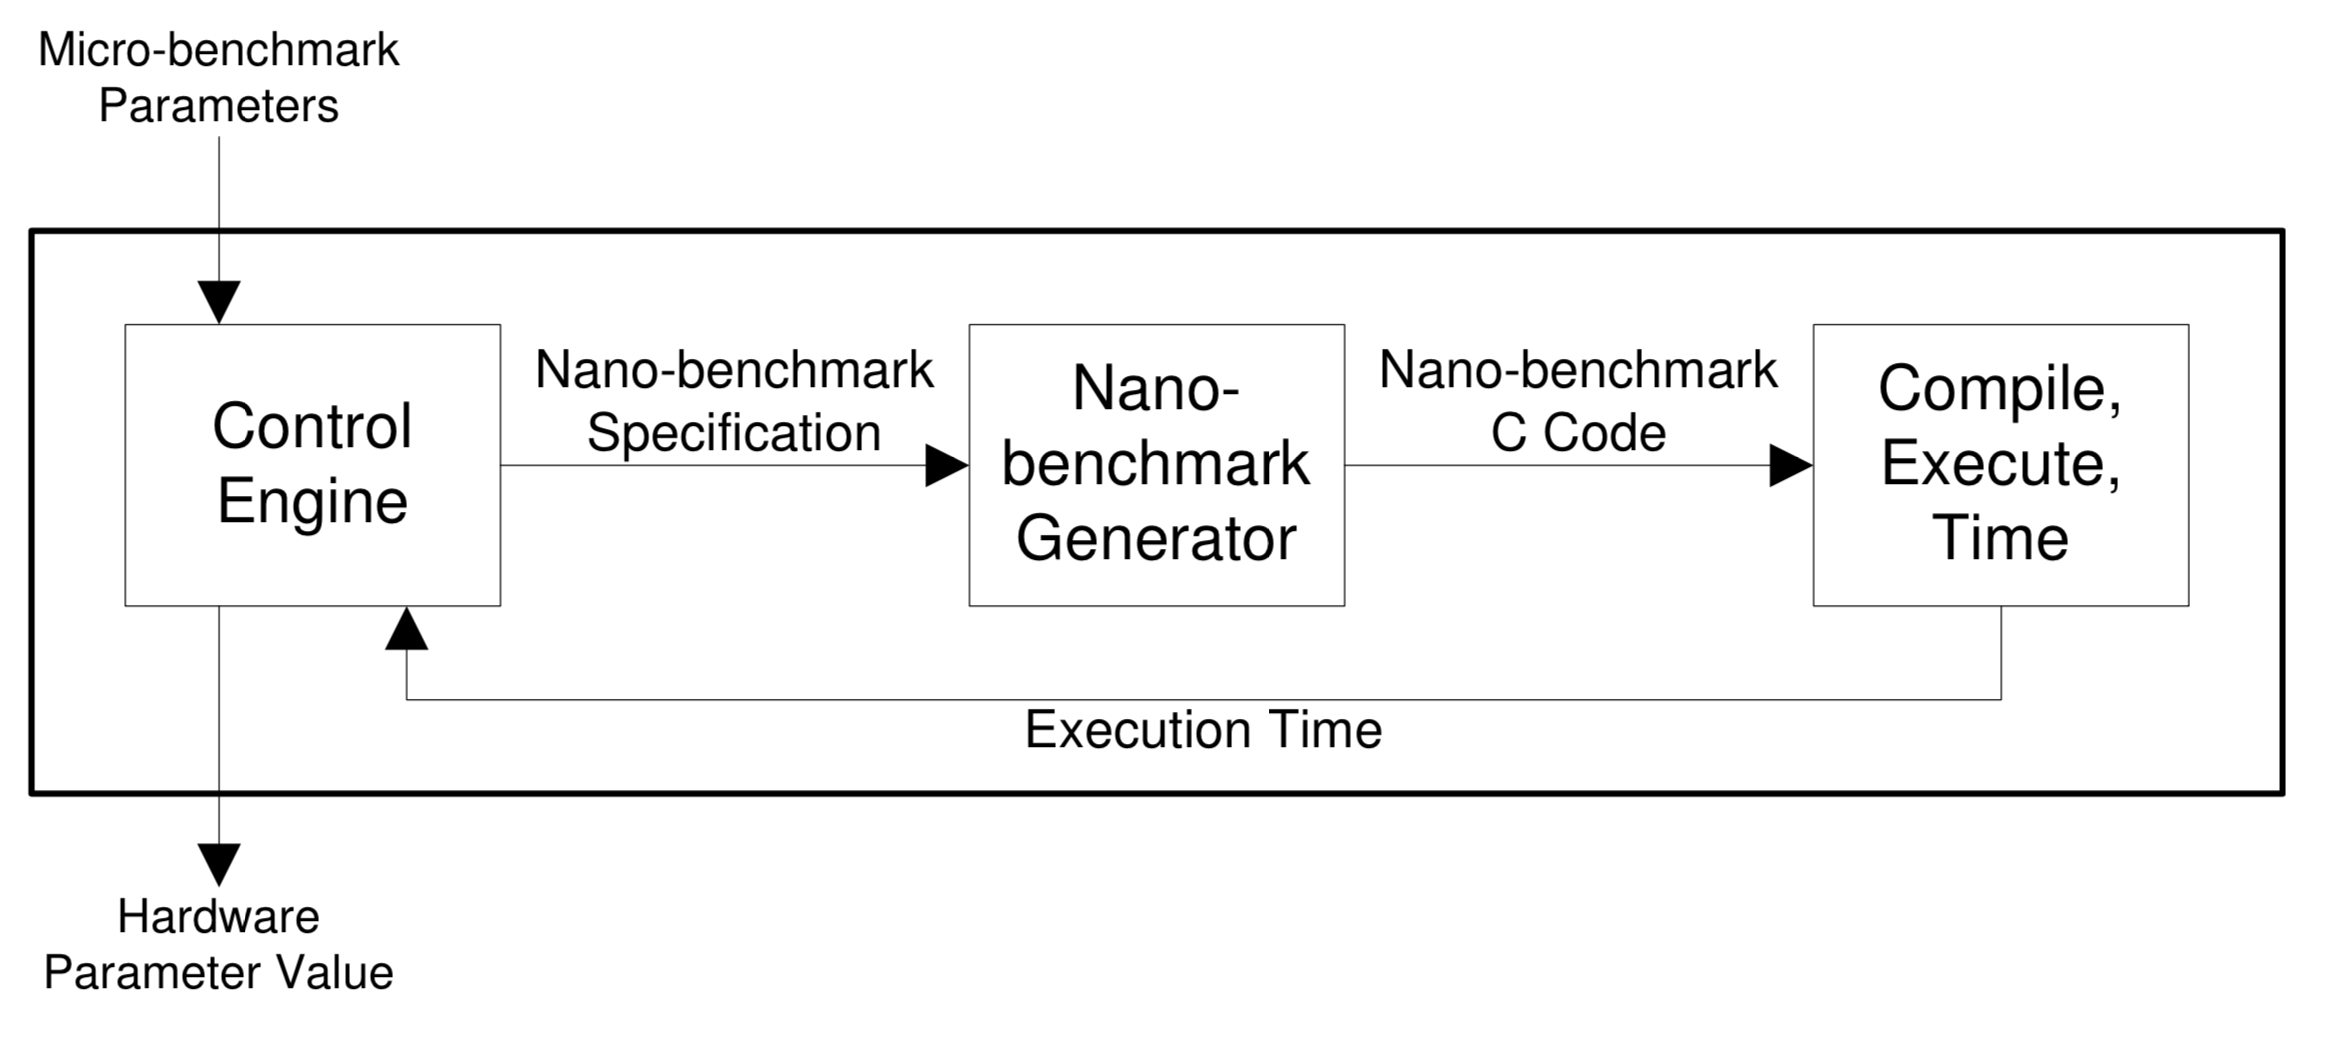
\includegraphics[width=10cm]{images/bench_xray.png}
    \caption{ Structure d'un micro-benchmark réalisé grâce à X-Ray  \cite{Yotov2004}.
    \label{pic_bench_xray}}
\end{figure}


\paragraph{P-Ray \cite{Duchateau2008}.} Dans le but de permettre à certaines librairie (ATLAS, SPIRAL ou FFTW) de s'auto-optimiser P-Ray permet de mesurer certains paramètres matériels. De la même façon que X-Ray et LMbench, l'apport de P-Ray permet de trouver ces spécifications pour des processeurs multi-coeurs. P-Ray permet de décrire la répartition des caches entre les coeurs, la topologie d'interconnexion des processeurs ainsi que les mécanismes de cohérence de caches. Leurs expérimentations montrent des résultats très précis comme la mesure de la latence de communication entre deux coeurs à travers le cache L3, L2 ou entre deux processeurs. Un effort particulier a été apporté pour éviter des optimisations du compilateurs et du prefetcher pouvant altérer les performances mesurées. Le benchmark de P-Ray a hérité d'un problème de X-Ray rendant impossible la portabilité du code entre différent systèmes d'exploitation. L'allocation mémoire suppose que toute les adresses physique soient contigues et cette caractéristiques dépend du système d'exploitation (les pages larges pouvant ne pas être disponibles).
Le code de P-Ray n'est cependant pas libre de droit.

\paragraph{Servet \cite{gonzalez2010servet}.} La suite Servet permet de mesurer certaines caractéristiques matériels telles que la hiérarchie de cache (taille, partage entre les coeurs) ou la bande passante mémoire. Ce travail ajoute a X-Ray et P-Ray des mesures des paramètres d'interconnexion pour la communication d'une mémoire distribuée ainsi qu'une méthodologie et une nouvelle technique de mesure. Une suite de benchmark permet aussi d'évaluer où se formeront les goulots d'étranglements lorsque plusieurs coeurs accèdent à la mémoire centrale. Enfin, Servet mesure la distance entre les coeurs en mesurant la latente de communication permettant à une application de placer plus efficacement les processus sur les différents coeurs.




\paragraph{Likwid}
\textbf{TODO}

Runs in user-space. Uses common kernel interfaces or perf_event
 Counts per HW thread (knowledge about processes)
 Derives metrics out of raw counter values

https://www.tdx.cat/bitstream/handle/10803/666955/TMR1de1.pdf?sequence=1

 A Toolset for performance-oriented developers/users
 Get system topology
 Place threads according system topology (affinity domains)
 Run micro-benchmarks to check system features
 Measure hardware events during application runs
 Determine energy consumption
 Manipulate CPU/Uncore frequencies


The LIKWID tool suite [17] includes the likwid-bench microbenchmarking framework, which provides a set of assembly language kernels. They cover a vari- ety of streaming access schemes. In addition the user can extend the framework by writing new assembly code loop bodies. likwid-bench takes care of loop counting, thread parallelism, thread placement, ccNUMA page placement and performance (and bandwidth) measurement. It does not, however, perform hardware event count- ing. For the HPM measurements we thus use likwid-perfctr, which is also a part of the LIKWID suite. It uses a simple command line interface but provides a comprehensive set of features for the users. Likwid-perfctr supports almost all interesting core and uncore events for the supported CPU types. In order to relieve the user from having to deal with raw event counts, it supports performance groups, which combine often used event sets and corresponding formulas for computing de- rived metrics (e.g., bandwidths or FLOP rates). Moreover, likwid-perfctr pro- vides a Marker API to instrument the source code and restrict measurements to certain code regions. Likwid-bench already includes the calls to the Marker API in order to measure only the compute kernel.





~\\

\subsubsection{Les benchmark mémoire}
%%%%%%%%%%%%%%%%%%%%%%%%%%%%%%%%%


\paragraph{lmbench \cite{HPC:lmbench}} Lmbench is a suite of portable benchmarks used to measure important characteristics of the memory such as bandwidth, memory latency and performance of the different cache levels.

\paragraph{Calibrator}


\paragraph{Saavedra} Ce benchmark est un des plus connus pour caractériser la mémoire. Il utilise une stride fixée pour accéder aux éléments d'un tableau. Le temps nécessaire à ces acces permet de déduire la taille des niveaux de la hiérarchie. Les expérimentations utilise des couples de $\{taille de tableau, taille de stride\}$. La taille du tableau augmente jusqu'à atteindre la taille du cache mesuré. La taille des strides est limitée a des tailles de puissance de 2 et ne dépassera jamais la taille du cache. Le tableau est ainsi parcouru pendant au moins une seconde. Comme le souligne \cite{Yotov2005} le problème d'une telle approche est de vouloir mesurer tout les niveaux de la hiérarchie simultanément. Les mesures peuvent alors être influencées par différents paramètres de différents niveaux de caches. Ces mesures doivent être interprétés par l'utilisateur, le programme ne créant pas automatiquement la hiérarchie. La lecture et l'écriture son réalisés sur la même données pouvant introduire des conflits dans le tampons d'écriture  \cite{Yotov2005}. Le benchmark assume que les donnés sont continues en mémoire mais n'utilise pas de pages larges.


\paragraph{X-ray}
Le travail \cite{Yotov2005} utilise X-Ray pour implémenter des micro-benchmarks pour mesurer la capacité, l'associativité, la taille des blocs ainsi que la latence de chaque niveaux de la hiérarchie de cache ainsi que du TLB. Contrairement aux benchmarks existants, l'outil mesure un niveau à la fois lui permettant d'être plus précis que les approches traditionnelles (X-Ray, Calibrator, lmbench et MOB). Utiliser X-Ray pour implémenter leur benchmark leur permet de mesurer la fréquence du processeur ansi que la latence et le débit instructions. Malheureusement, le code de X-Ray n'a pas été maintenu et n'est plus disponible au téléchargement.


\paragraph{STREAM} Le code STREAM permet de mesurer la bande passante mémoire atteignable grâce à l'implémentation de quatre noyaux: COPY ($c=a$), SCALE ($b=\alpha \times c$), ADD ($c=a+b$) et TRIAD ($a=b+\alpha \times c$).


The second worldwide known benchmark is STREAM \cite{HPC:stream} that was originally developed to understand the performance differences between two architectures for a weather application.

The main problem with those benchmarks comes from their artificial code not representing real application. To this end, other specific benchmarks have been developed to reflect how real application would perform. On recent HPC architectures, having a good HPL performance is no longer correlated with having good performance with real applications, so the HPCG was introduced \cite{HPC:hpcg}. 

\paragraph{HPCG} This benchmark fills the gap by implementing some micro-benchmarks more representative of the workload used in the industry as sparse matrix-vector multiplication or sparse triangular solvers.




    \paragraph{STREAM}
        Le benchmark STREAM est surement un des benchmarks les plus connus et les plus utilisé au monde. Il a été développé et est maintenu par John McCalpin surnommé "Dr. Bandwidth". Le benchmark mesure la bande passante soutenanble pour quatre noyaux vectoriels simples. Les résulats sont donnés en GB/s et contiennent à la fois les opérations de lecture et d'écriture. Pour ces quatre opérations STREAM fonctionne en générant un tableau de nombres aléatoires d'une taille spécifiée (qui est ensuite stocké en RAM) et effectue quatre types d'opérations: \textit{copy, scale, add, triad}.  Le benchmark utilise \textit{OpenMP} pour utiliser la totalité des coeurs disponibles. Ces différents tests étaient à l'origine destinés pour caractériser la performance des architectures vectorielle. La performance mémoire pouvait alors varier d'une opération à l'autre. Aujourd'hui, la performance calculatoire des architectures n'est plus la contrainte principale et les quatre micro-benchmark obtiennent des performances équivalentes. Il est généralement accepté que la mesure donnée pour l'opération de \textit{triad} correspond à la bande passante maximale atteignable par l'architecture. On remarque que le noyeau de calcul du \textit{triad} est relativement simple et ne consiste qu'en la lecture de deux éléments et l'écriture du résultat. Les applications réelles utilisant des motifs d'accès bien plus complexes, cette mesure n'est pas représentative de la performance réellement atteignable par celles-ci \footnote{\url{https://www.intel.ru/content/dam/doc/white-paper/resources-xeon-7500-measuring-memory-bandwidth-paper.pdf}}
        

    \paragraph{lmbench} 
        Le benchmark \textit{lmbench}\cite{Staelin2004} a été développé par deux ingénieurs des HP Labs d'Israel en 2004. Ce code est en fait une suite de micro-benchmark permettant de mesurer la performance de plusieurs aspects d'une architecture: lecture d'un jeu de données, ouverture de fichiers, création de pipe, fréquence mémoire, taille d'une ligne de cache, taille de la TLB, bande passante mémoire (Stream). L'ensemble des codes peut être exécuté pour caractériser la mémoire d'un système partagé ou distribué \cite{Staelin2002}.
        \textit{Lmbench} facilite l'ajout de nouveau micro-benchmarks et mesure leur performance en donnant la latence par instruction et le débit mémoire. Le framework s'occupe de leur exécution pour atteindre des mesures de performances ayant une performances d'au moins 1\%. Écrit en ANSI-C et respectant la norme POSIX le benchmark a été développé pour maximiser sa portabilité. Cependant, sa compilation sur des architectures récentes peut être plus difficile \cite{Yotov2004}. En raison de son incapacité à mesurer les performances du cache distant et les transactions de cohérence du cache, le benchmark \textit{x86-membench} benchmark \cite{Molka2017b} a été développé pour supporter la mesure de la bande passante et de la latence du cache local ou distant mais aussi de la mémoire. Le benchmark n'utilise aucune méthode de parallélisme empêchant une caractérisation poussée des architectures modernes. 
        
    
    \paragraph{P-ray} 
        Pour remédier à l'incapacité de \textit{lmbench} de caractériser les plateformes multi-coeurs, le benchmark P-ray a été développé \cite{Duchateau2008}. Pour cela il étend les micro-benchmarks existant pour trouver le niveau des caches partagés, la topologie d’interconnexion, la bande passante effective ou la taille des blocs pour la gestion de cohérence des caches. Pour éviter les optimisations du compilateur (\textit{pointer chaising}), le benchmark utilise un système de liste chaînée lors de l'initialisation. Les résultats obtenus sont eux très précis et s'approchent souvent des maximums théoriques attendus.

    \paragraph{X-Ray} X-RAY \cite{Yotov2004} est un \textit{framework} utilisé pour implémenter des micro-benchmark destinés à mesurer des paramètres utile pour l’auto-optimisation. Pour cela il génère plusieurs benchmark gràce à un framework \textit{Nano-benchmark Generator}. Cette génération est dynamique car les benchmarks à générer varient en fonction de ceux déjà exécutés. Par exemple, le calcul de latence à besoin de connaître la fréquence du processeur pour donner un résulat en cycles

    Un objectif des benchmarks est de mesurer les performances maximales atteignables par une plate-forme. Ainsi, il est possible de quantifier la performance d'une application réelle en la comparant à cette première valeur. Le système mémoire étant le goulot d'étranglement de la performance d'une majorité d'application, de nombreux travaux ont été réalisés pour sa caractérisation et son optimisation. Un benchmark très connu (STREAM) permet de mesurer la bande passante maximale atteignable par 4 kernels de calculs différents. Il est donc possible d'utiliser ces résultats pour analyser la performance d'applications utilisant les mêmes familles d'algorithmes.


   Il existe de nombreux benchmarks permettant de caractériser différentes parties du système mémoire: les accès mémoires concurrents de systèmes multi-processeurs\cite{Mandal2010}, polices de mappage mémoire des systèmes NUMA \cite{Diener2015}, prédiction de la bande passante mémoire en fonction du placement des coeurs \cite{Wang2016a}, caractérisation de la hiérarchie mémoire \cite{Cooper2011}.
    
  

\newpage

\subsection{Modélisation de performances}


\subsubsection{Modèle du Roofine} \label{sec:roofline}
%%%%%%%%%%%%%%%%%%%%%%%%%%%%%%%%%%%%%%%%%%%%%%%%%%%%%%%%%%%%%%%%%%%

%%%%%%%%%%%%%%%%%
\paragraph{Motivation et objectifs}
%%%%%%%%%%%%%%%%%
Présenté par William et al. en 2009 \cite{Williams2008}, le modèle du \textit{roofine} est un modèle de performance simple qui représente graphiquement les performances d’un code en situant sa performance par rapport au performances maximales de l’architecture. L’objectif principale de ce modèle est de donner le pourcentage de la performance disponible atteinte par un code. L’intérêt de ce model est de restreindre l’analyse de performance aux deux ressources importantes pour les applications HPC: la performance calculatoire (GFLOP/s) et la performance du bus mémoire (GB/s).
Le modèle est utilisé pour représenter les différentes fonctions clefs d’une application. Ainsi, le programmeur pourra commencer son travail d’optimisation sur les fonctions avec le plus de potentiel.

\begin{figure}
    \center
    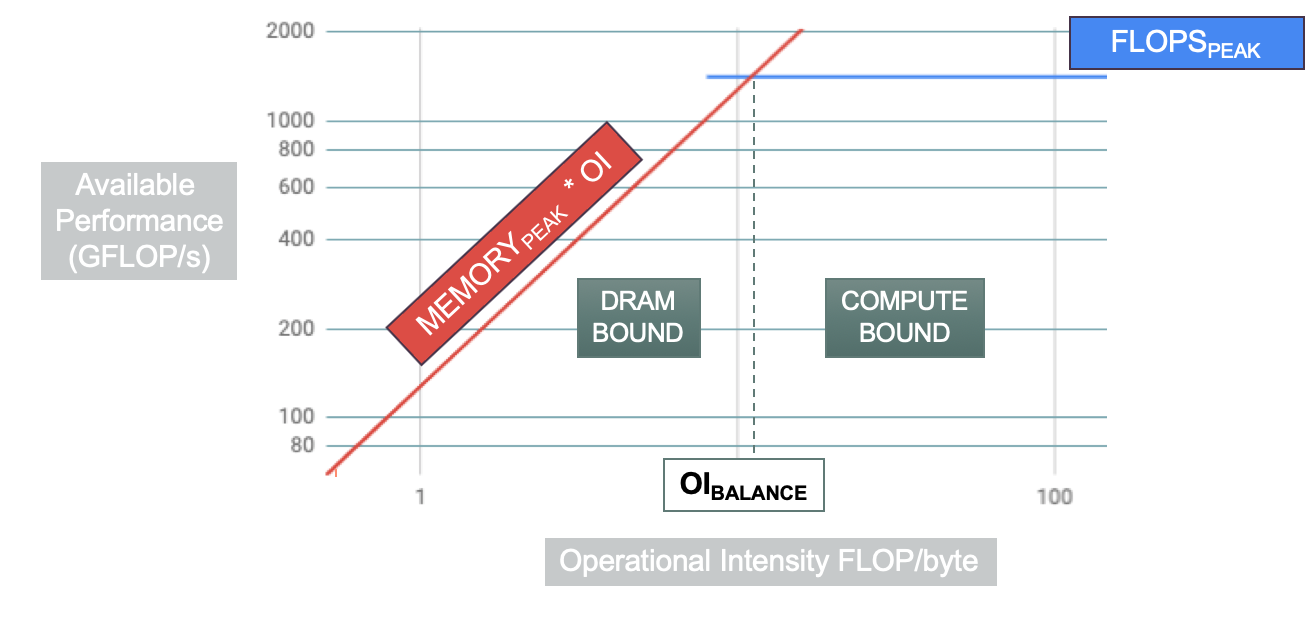
\includegraphics[width=10cm]{images/roofline.png}
    \caption{\label{fig:roofline} Représentation graphique du modèle du \textit{roofline}. En fonction de son l'intensité opérationnelle, la performance d'un code sera limitée par la bande passante ou par le processeur.}
\end{figure}


La \autoref{fig:roofline} montre une représentation du modèle du \textit{roofine}. Sur l’axe des abscisse est représentée l’intensité opérationnelle de l’algorithme (en flops/byte) qui correspond nombre d’opération flottante appliqué à chaque byte de donnée amené depuis la mémoire. Sur l’axe des ordonnées est représentée la performance de calcul mesurée en GFLOP/s.
Chaque hot spot sont placés en fonction de leur intensité opérationnelle, calculée à partir de la lecture du code, et de sa performance, mesurée lors de l’exécution.

%%%%%%%%%%%%%%%%%
\paragraph{Preuve et construction}
%%%%%%%%%%%%%%%%%
L’objectif du modèle est de déterminer si la performance du code pour une architecture donnée est structurellement limité par la performance du processeur ($FLOPS_{peak}$ en $GFLOP/s$) ou bien par la performance du bus mémoire ($MEMORY_{peak}$ en $GB/s$). Une application réalisant la lecture de deux nombres pour y réaliser des centaines d’opérations verra ses performances limitées par la capacité de calcul $FLOPS_{peak}$ du processeur. Inversement, une application devant lire un grand jeu de données pour ne réaliser qu'une opération sur chaque valeur, verra ses performance limitées par celle du bus mémoire $MEMORY_{peak}$. On peut estimer la quantité de calculs à réaliser sur chaque donnée en calculant son Intensité Opérationnelle  ($\text{OI}$ en $flop/byte$). Pour cela il faut lire le code source pour compter manuellement le nombre d’opérations réalisées ($\text{\#FLOP}$) et le nombre de données nécessaires chargées depuis la mémoire ($\text{\#BYTE}$). On peut ainsi calculer l’Intensité Opérationnelle d’un code en faisant le ratio des deux valeurs.

\begin{equation}
\begin{aligned}
        \text{OI}_{kernel} =\ &\cfrac{\text{\#FLOP}}{\text{\#BYTE}}
\end{aligned}
\end{equation}

Le temps pour exécuter le code ($\text{TEMPS}_{theorique}$), sera le temps mis par la ressource la plus utilisée par le code. On peut estimer ce temps par la formule suivante.
\begin{equation}
\begin{aligned}
     \text{TEMPS}_{theorique} =\  &max 
     \begin{cases} 
        \quad \cfrac{\text{\#FLOP}}{\text{FLOPS}_{peak}}    \\[15pt]
        \quad \cfrac{\text{\#BYTE}}{\text{MEMORY}_{peak}}
    \end{cases}
\end{aligned}
\end{equation}




La performance théorique du code ($\text{PERF}_{theorique}$ en GFLOP/s) peut être calculée grâce aux transformations successives de l'\autoref{eq:PERFT}.
\begin{equation}
\begin{aligned}
\label{eq:PERFT}
\cfrac{\text{TEMPS}_{theorique}}{\text{\#FLOP}}  =\ &\text{max}
\begin{cases} 
    \cfrac {1}{\text{FLOPS\_{peak}}}    \\[15pt]  
    \cfrac {\cfrac{\text{\#BYTE}}{\text{MEMORY}_{peak}}}{\text{\#FLOP}} 
\end{cases}\\[20pt]
\cfrac{\text{\#FLOP}}{\text{TEMPS}_{theorique}}  =\ &\text{min}
\begin{cases} 
    \text{FLOPS}_{peak}    \\[15pt]  
    \cfrac{\text{\#FLOP}}{\text{\#BYTE}} \times \text{MEMORY}_{peak}
\end{cases}\\[20pt]
\text{PERF}_{theorique}  =\ &\text{min}
\begin{cases} 
    \text{FLOPS}_{peak}    \\[15pt]  
    \text{OI}_{kernel} \times \text{MEMORY}_{peak} 
\end{cases}
\end{aligned}
\end{equation}



Pour une architecture, il faut déterminer pour quelle intensité opérationnelle une application est limitée par la mémoire ou le processeur. Pour cela, il faut calculer l’intensité opérationnelle ($\text{OI}_{balance}$) correspondant au croisement des deux droites sur la \autoref{fig:roofline}. 

\begin{equation}
\begin{aligned}
 \text{FLOPS}_{peak} =\ &\text{OI}_{balance} \times \text{MEMORY}_{peak} \\[20pt]
 \text{OI}_{balance} =\ &\frac{\text{MEMORY}_{peak}} {\text{FLOPS}_{peak}} 
\end{aligned}
\end{equation}

Une application dont l’intensité opérationnelle est inférieure à $\text{OI}_{balance}$ verra sa performance limitée par le système mémoire. Plus rarement, si l’intensité opérationnelle d’une application est supérieure à $\text{OI}_{balance}$, la performance sera alors limitée par le processeur.

\paragraph{Construction}
La première étape dans la construction du graphique est de tracer les deux axes limitant les performances d’un code. Ces deux droites représentes les performances crêtes de la mémoire et du processeur. Pour obtenir ces valeurs, elles peuvent être calculées à partir des spécifications du processeurs. Cependant, avec la complexification des architectures, il est difficile de les atteindre même avec des benchmarks prévus à cet effet. Il est donc préférable de les représenter par des valeurs mesurées comme indiqué dans la littérature  \cite{farjallah2014preparing}. Pour la mémoire le benchmark Stream peut être utilisé. Pour la performance du processeur, nous utilisons le générateur de benchmark présenté dans la \autoref{sec:kg}. D’autres travaux sont venus compléter les benchmarks disponibles pour caractériser l’architecture \cite{lo2014roofline}.




%%%%%%%%%%%%%%%%%
\paragraph{Évolutions}
%%%%%%%%%%%%%%%%%


Le \textit{roofine} a reçu de nombreuse améliorations depuis sa création. En 2014, les travaux \cite{Ilic2014} constate que le modèle originale n’est pas suffisament précis à cause de la faible précision de caractérisation de l’architecture. En effet, un code pouvant profiter de la localité des données dans les caches pourrait atteindre des performances supérieur au maximum prévu par le modèle utilisant seulement le bande passante mémoire. Inversement, la performance crête est calculé pour un code utilisant tous les coeurs du processeur, avec des instructions FMA vectorisées. Cependant, par leur nature, certain code ne peuvent pas utiliser ces  caractéristiques. La performance crête étant alors impossible à atteindre. Le modèle Cache-Aware Roofline Model (CARM) \cite{Ilic2014} a ainsi été développé permettant de représenter la performance des différents niveaux de caches. Cependant, le programmeur doit comprendre si son application peut tirer partie de cette localité, ce qui peut rendre cette approche plus difficile. Le modèle à depuis été affiné avec le Locality Aware Roofline Model (LARM) \cite{Denoyelle2018} permettant de modéliser les accès en mémoire non uniforme (NUMA).
D’autres travaux essaient d’automatiser sa construction \cite{lo2014roofline} pour faciliter son usage. L’outil de profiling d’Intel a intégré les modèles CARM et LARM pour automatiser la recherche des hot spot et afficher leur performance sur un même graphique. Pour cela, il désassemble le code et calcule l’intensité opérationnelle de la boucle étudiée.


%%%%%%%%%%%%%%%%%
\paragraph{Critiques}
%%%%%%%%%%%%%%%%%

La force de cette approche est de montrer rapidement au programmeur si son application est efficace ou non. Dans le cas échéant, il sait s’il doit travailler sur l’optimisation des flops ou de la mémoire. En modélisant les principaux kernels de son application, le programmeur saura sur lesquels ses optimisations seront le plus bénéfiques.

Bien d’ayant reçu de nombreuses améliorations, ce modèle doit être utilisé pour commencer l’analyse de performance. Mais il ne permet pas de modéliser n’y de comprendre finement la raison d’une performance.
La majorité des applications étant limitée par la bande passante mémoire, il est rare d’utiliser ce modèle pour modéliser la performances des unités de calculs. Mais il peut être intéressant de calculer l’intensité opérationnelle d’une boucle pour s’en assurer avant d’apporter des optimisations. De plus, les accélérateurs à venir essaient de réduire le trou de performance entre les processeurs et la mémoire. Cette modélisation est donc importante pour l’analyse de performance.


\newpage


\section{Conlusion}\label{sec:conclusion-hpc}


\printbibliography[heading=references,segment=\therefsegment]


Référence:
- These - Contribution à l’amélioration des méthodes d’optimisation de la gestion de la mémoire dans le cadre du Calcul Haute Perf.pdf

 
https://patents.google.com/patent/US9111032B2/en  
    -A bottleneck is a region of a program (e.g., program code) where significant execution time is spent. Typically, software developers use a profiling tool to collect program execution profiles such as the timing information for each method, routine, process, etc. With the help of such a profiling tool, the developer can sort, e.g., methods by the time spent on them. The methods that consume an amount of time greater than a threshold defined by, e.g., the developer may be treated as bottlenecks. However, the effectiveness of this approach depends on the program's runtime characteristics. Many programs, such as large enterprise commercial applications, do not have obvious bottlenecks. Therefore, their profiles contain a large amount of routines, processes, or methods where the execution time is spent relatively evenly (e.g., within a threshold). This type of profile is often referred to as a “flat profile” because no method dominates the execution time.
    